% !TeX spellcheck = en_US
\documentclass[a4paper]{report}
\usepackage{geometry}
\geometry{a4paper,top=4cm,bottom=4cm,left=3.5cm,right=3.5cm}%
\usepackage{graphicx}
\usepackage[english]{babel}
\usepackage[utf8]{inputenc}
\usepackage[T1]{fontenc}
\usepackage{float}
\usepackage{siunitx}
\usepackage{textcomp}
\usepackage{float}
\usepackage{subfig}
\usepackage[colorinlistoftodos]{todonotes}
\usepackage{amsmath}
\usepackage{array}
\usepackage{bm}
\usepackage{comment}
\usepackage[pdf]{graphviz}
%\usepackage{pslatex}
%\usepackage{biblatex}
%
%sudo apt install graphviz
%
%dot -Tpdf testdot.gv -o testdot.pdf
%
%
%

\begin{document}
	
	\begin{titlepage}
		\centering
		
\includegraphics[width=0.2\textwidth]{img/logo_unito.JPG}\par
		\vspace{1cm}
		{\scshape\LARGE Physics Department of Turin \par}
		{\scshape\LARGE Master's degree course in physics \par}
		\vspace{4cm}
		{\Huge \textbf{Development and test of FPGA firmware extensions for the configuration and readout of the new ABACUS\_v2 chip for beam~monitoring applications in hadron therapy} \par}	
		\vspace{3cm}
		{\Large\itshape Academic year 2020/2021\par}
		\vspace{1cm}
		{\large Candidate: Stefan Cristi Zugravel \par} 
		{\large Supervisor: Dott. Luca Pacher \par}
		{\large Co-Supervisor: Prof. Vincenzo Monaco \par}
		
		\vfill
		
		{\large \today\par}
	\end{titlepage}

	%\begin{center}
	%{\Huge \textbf{Abstract}}
%\end{center}
%\vspace{2cm}

\chapter*{Abstract}
\addcontentsline{toc}{chapter}{Abstract}
\thispagestyle{plain}
Hadron therapy is a type of oncological radiotherapy for the treatment of solid tumors that uses proton or
ion beams instead of conventional X-rays. The usage of hadron particles allows a better control on the energy release,
improving the precision of the treatment and the conservation of healthy tissues around the target.
Particle beams are obtained by means of dedicated accelerators, requiring a precise control of particle flux and beam profile.
Thus beam-monitoring systems become of primary importance, demanding the usage of fast particle sensors and readout electronics to monitor
in real-time the particle beam reaching the patient.\\

\noindent In this context the Medical Physics group at University of Turin and INFN (the Italian National Institute for
Nuclear and Particle Physics) is participating to the MoVeIT (Modeling and Verification for Ion beam Treatment planning) research project, which aims to develop new and
innovative models for biologically optimized Treatment Planning Systems (TPS) using ion beams in hadron therapy.
As part of the project the Turin group is involved in the development of solid state detectors and custom readout electronics for measuring with high precision
the characteristics of the hadron beam before and during the irradiation, such as number of particles delivered per unit time, energy and beam profile.\\

\noindent Low-Gain Avalanche Diode (LGAD) thin silicon sensors segmented in strips have been selected as a promising choice for the implementation
of the final beam-monitoring system. Thanks to the internal gain mechanism this sensor technology allows to obtain a large
Signal-to-Noise Ratio (SNR) for very low amounts of deposited charge. This allows to detect and count single beam particles.

\noindent Silicon strips are read out by a full-custom and optimized Application Specific Integrated Circuit (ASIC) designed by Turin INFN.
The chip, named ABACUS (Asynchronous-logic-Based Analog Counter for Ultra fast Silicon strips), has been 
designed using a commercial CMOS 110~nm technology and integrates 24 readout channels. Each channel includes a low-noise charge preamplifier 
and a fast discriminator. The external data acquisition system uses commercial Field Programmable Gate Array (FPGA) boards that receive
the data from up to 6 readout chips.\\% A second version of the chip, refered as ABACUS2 \\

\newpage
\thispagestyle{plain}
\noindent This thesis presents my personal contributions on the upgrade of the FPGA firmware used to characterize
the second version of the ABACUS chip and measurement results, referred as ABACUS2.
The FPGA used to readout the chip is a Kintex-7 KC705 board by Xilinx programmed using the VHDL Hardware Description Language.
The FPGA is responsible for both the chip configuration and data readout.

\noindent The first part of my work describes the upgraded VHDL firmware, which includes several new features such as:
i) the creation of a debugging tool for malfunctioning channels on the FPGA board;
ii) the complete rewriting of the internal Digital to Analog Converter (DAC) configuration system for the new ABACUS chip, which
now uses an address-based system with an I2C controller instead of a serial method (I2C protocol);
iii) the implementation of a latch for internal counters;
iv) the addition of a timestamp generator for a more accurate calculation of the particle rate.
\newline
The second part of the thesis presents obtained experimental results that validated the new FPGA firmware extensions.
Measurements include threshold scans studies to quantify the threshold dispersion between channels and rate calculations.
\vspace{1cm}
\newline
This thesis is organized as follows:
\vspace{0.25cm}
\newline
Chapter 1 describes the physical mechanisms and advantages of hadron-therapy compared to conventional radiotherapy. The most advanced dose distribution systems and the detectors used are described.
\vspace{0.25cm}
\newline
Chapter 2 describes the devices developed within the MoVeIT project for dose monitoring.
In particular it is shown the operating principle of the LGAD sensors used and their advantages for the application under study.
The characteristics of the chip developed by the INFN section of Turin for the amplification and discrimination of signals are also described.
\vspace{0.25cm}
\newline
Chapter 3 contains a brief history of the FPGA, its main components and a comparison with ASICs and others programmable devices.
After that there is a short introduction to the hardware description languages and the associated design workflow.
There is a brief discussion on the tools used for the development and lastly it is described the FMC debug tool that I implemented.
\vspace{0.25cm}
\newline
Chapter 4 contains a description of the FPGA firmware and a detailed explanation of the implemented extensions, which are: the trimming DACs configuration logic, the counter latch system and of the timestamp generator.
For each new addition software simulation and considerations on the implemented design are included.
\vspace{0.25cm}
\newline
Chapter 5 describes the hardware devices involved in the project such as the test setup, the test board and the voltage translator.
For each addition to the firmware tests on board have been performed and described.

	
	\tableofcontents
		
	\part{Introduction to the MoVe\_IT project}
\chapter{Hadron Therapy}

\section{Introduction}
The National Cancer Institute define a tumor\cite{tumor} as “an abnormal mass of tissue that results when cells divide more than they should or do not die when they should”.
In a healthy body, cells grow, divide, and replace each other in the body. As new cells form, the old ones die. When a person has cancer, new cells form when the body does not need them. If there are too many new cells, a group of cells, or tumor, can develop.
A tumor develops when cells reproduce too quickly. Tumors can vary in size from a tiny nodule to a large mass, depending on the type, and they can appear almost anywhere on the body.
There are three main types of tumor:
\begin{itemize}
\item \textbf{Benign}: These are not cancerous. They either cannot spread or grow, or they do so very slowly. If a doctor removes them, they do not generally return.
\item \textbf{Premalignant}: In these tumors, the cells are not yet cancerous, but they have the potential to become malignant.
\item \textbf{Malignant}: Malignant tumors are cancerous. The cells can grow and spread to other parts of the body.
\end{itemize}
Radiation therapy is the medical use of ionizing radiation to treat cancer. In conventional radiation therapy, beams of X rays (high energy photons) are produced by accelerated electrons and then delivered to the patient to destroy tumour cells. Using crossing beams from many angles, radiation oncologists irradiate the tumour target while trying to spare the surrounding normal tissues. Inevitably some radiation dose is always deposited in the healthy tissues.
When the irradiating beams are made of charged particles (protons and other ions, such as carbon), radiation therapy is called hadron therapy\cite{radiationtherapy}. The strength of hadron therapy lies in the unique physical and radiobiological properties of these particles; they can penetrate the tissues with little diffusion and deposit the maximum energy just before stopping. This allows a precise definition of the specific region to be irradiated. The peaked shape of the hadron energy deposition is called Bragg peak and has become the symbol of hadron therapy. With the use of hadrons the tumour can be irradiated while the damage to healthy tissues is less than with X-rays.

\section{Interaction between matter and charged particles}
Charged particles with mass greater than the one of the electron lose energy in matter through ionization.
A classic calculation for the energy lost in ionization can be done taking into account two assumptions:
\begin{itemize}
	\item the speed of the atomic electron is negligible compared to the one of the incident particle;
	\item the mass of the incident particle is big in relation to the target mass. This means that the incident particle for each single hit receives a small amount of momentum and thus the direction of flight does not changes.  
\end{itemize}
\noindent This hypothesis is valid keeping into consideration that the mass of the electron is 0.51 MeV, a muon has mass 105.6 MeV, for a proton it is 938.2 MeV and for a carbon ion ${}^{12}$C it is 11177.9 MeV.
\newline
The classic calculation results in the Bethe-Block formula in equation \ref{eq:bethe} that describes the average energy loss in the target for unit of length, also called stopping power.
\begin{equation}\label{eq:bethe}
	-\dfrac{\mathrm dE}{\mathrm dx} = 2 \pi N_{a} r_{e}^{2} m_{e} c^{2} \rho \dfrac{Z}{A}  \dfrac{z^{2}}{\beta^{2}}\left[\ln\left(\dfrac{2m_{e} \gamma ^{2} v^{2} W_{max}}{W^{2}}\right) - 2\beta^{2} - \delta 2\frac{C}{Z}\right]
\end{equation}
\noindent In equation \ref{eq:bethe}:
\begin{itemize}
	\item $N_a$: is the Avogadro number;
	\item $r_e$: is the classical radius of the electron;
	\item $m_e$: is the mass of the electron;
	\item $\rho$: target density;
	\item $Z $: target atomic number;
	\item $A $: target atomic mass;
	\item $W $: target average ionization energy;
	\item $z $: incident particle charge;
	\item $W_{max} $: maximum energy transferred in a collision; 
	\item $\delta $: polarization parameter in target
	\item $c/z $: core electrons shielding parameter 
	\item $\beta = v/c $
\end{itemize}
\noindent The stopping power depends by the target mass, atomic number, density and average ionization energy (A, Z, $\rho$, W). To overcome and eliminate this dependence it was defined the massic stopping power in equation \ref{eq:stoppingpower} that is measured in MeV/(g cm${}^2$)
\begin{equation}\label{eq:stoppingpower}
	\delta = - \frac{1}{\rho} \frac{dE}{dx}
\end{equation}
\noindent In figure it can be seen the trend of the massic stopping power of a $\mu^+$ passing through a copper layer.
\begin{figure}[H]
	\centering
	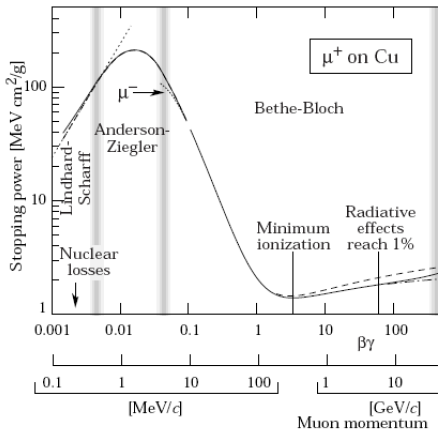
\includegraphics[width=0.7\linewidth]{IMG/ch1/MassicStoppingPower}
	\caption{Massic Stopping power in function of the $\mu^+$ momentum passing through a copper layer}
	\label{fig:massicstoppingpower}
\end{figure}
\noindent In the trend of the stopping power in function of the momentum can be noted a de-growth for low momentum values that is due to the term $\frac{1}{\beta^2}$ in equation \ref{eq:bethe}; the stopping power decreases until it reaches a minimum, and then slowly grows back.
\newline
The average path (range) of a charged particle can be calculated by integrating the stopping power along the "walk".
\begin{equation}\label{eq:range}
	R=\int_{E_i}^{0} \frac{1}{\frac{dE}{dx}}dx
\end{equation}
\noindent The range depends approximately on the A / Z ratio of the material and grows approximately with the square of the initial kinetic energy of the charged particle. The accrual
of energy loss increases as the kinetic energy of the particle decreases with the depth of penetration, with a rapid ascent at the end of the path. The density of ionization of the charged particles along their path in the medium is therefore
characterized by a plateau followed by a pronounced maximum towards the end of range, called Bragg peak, which is located at an energy-dependent depth initial kinetics of the incident particle, as shown in figure \ref{fig:braggpeak}.
If more particles are considered then it should be kept in mind
the statistical fluctuations on the collisions of the particles and on the energy transferred for each collision: these fluctuations are well described by the Landau distribution \cite{landau}
, generate uncertainty about the distance reached by the particles ("straggling"). Beyond all these considerations we must not neglect the possible interactions with the nuclear components of the matter crossed. One effect is enlargement
lateral of the beam due to the interaction with the Coulomb fields of the nuclei that it is inversely proportional to the mass of the incident particle. The second effect it is due to the fragmentation of the primary bundle and/or of the nuclei of the material passed through due to nuclear interactions. The fragmentation cross section becomes relevant for ions heavier than the proton, such as carbon ions or heavier, and causes a decrease in the number of particles incident along the path
and the development of secondary fragments. The fragments produced deposit theirs energy deeper than the Bragg peak giving rise to a queue in the distribution.
\begin{figure}[H]
	\centering
	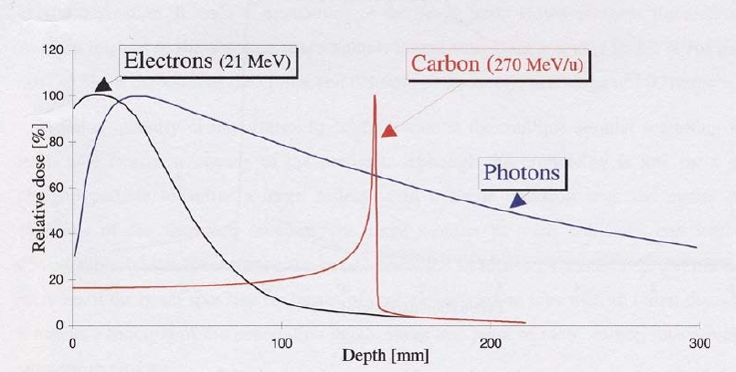
\includegraphics[width=0.7\linewidth]{IMG/ch1/BraggPeak}
	\caption{Dose profile for a 21MeV electron, 270MeV/u carbon ion and photon beam}
	\label{fig:braggpeak}
\end{figure}  

%\begin{equation}\label{eq:bethe2}
%	W_{max} = \dfrac{2m_{e} c^{2} \eta^{2}}{1+2s \sqrt{1+\eta^{2}} + s^{2}};\qquad s=m_{e}/M;\eta=\beta\gamma.
%\end{equation}


\section{Effects of radiations on biological systems}
Radiation is energy. A charged particle when it interacts with the human body loses its energy. The measurement and calculation of the ionizing radiation dose absorbed by an object is called radiation dosimetry.
\newline
Thus the dose (D) can be defined as the energy absorbed divided by the object mass.
\begin{equation}\label{eq:dose}
	D\left[Gy \right] =\frac{dE}{dm}
\end{equation}
In the I.S. the unit of measure is the Gray(Gy)[JKg${}^{-1}$]=1J/1Kg.
\newline
It is also common the use of an equivalent dose (H=DxW$_1$) where W$_1$ is a weight that depends on the type of particle (photon, electron, neutron, proton, heavy charged particle, ecc...). The unit of measure of the equivalent dose is the Sievert(Sv)[JKg${}^{-1}$], although in the past it was used the rem[1Sv=100rem].
\newline
When monitoring the dose absorbed by an human body it must me considered that not every organ has the same resistance to radiation, thus it is used the effective dose (E=HxW$_2$) which is the equivalent dose multiplied by the weight W$_2$ which depends on the part of the body interested by the radiations.
\newline
\noindent The energy deposition is strictly dependent by the type of radiation like photons, electrons or heavy charged particles. As shown in figure \ref{fig:braggpeak} the relative dose percentage delivered by the photons is maximum at low depth and then has an exponential decrease as the thickness of the tissue increases.
The dose profile in function of the depth for heavy charged particles (as carbon ions) is characterized by a low dose at the beginning of the tissue and then by a extremely peaked spike at the end of their travel (Bragg peak).
Since the depth of this peak depends by the beam energy, this can be tuned to deliver the dose at different depths.
Moreover, thanks to the high mass of the particles, it is possible to greatly reduce the lateral diffusion effects thus saving the healthy tissues and the critical structures near the target.
\begin{figure}[H]
	\centering
	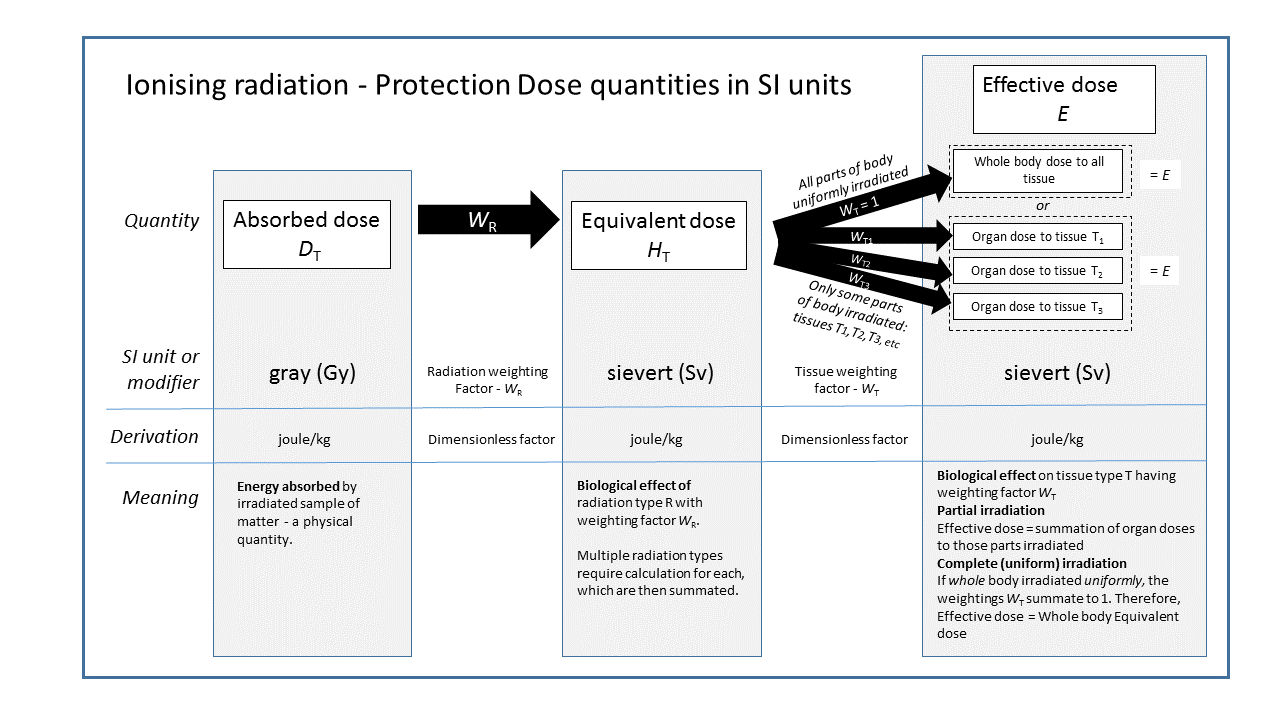
\includegraphics[width=0.7\linewidth]{IMG/ch1/SIRadiationDoseUnits}
	\caption{Absorbed, equivalent and effective dose units and meanings}
	\label{fig:SIRadiationDoseUnits}
\end{figure} 
\noindent With heavy charged particles is therefore possible to accurately focus the beam for a selected depth; this is not possible with other sources of radiation.
\newline
The different rates of energy loss at different depths for photons and heavy charged particles produce different dose distributions as shown in figure \ref{fig:Dose}.
\begin{figure}[H]
	\centering
	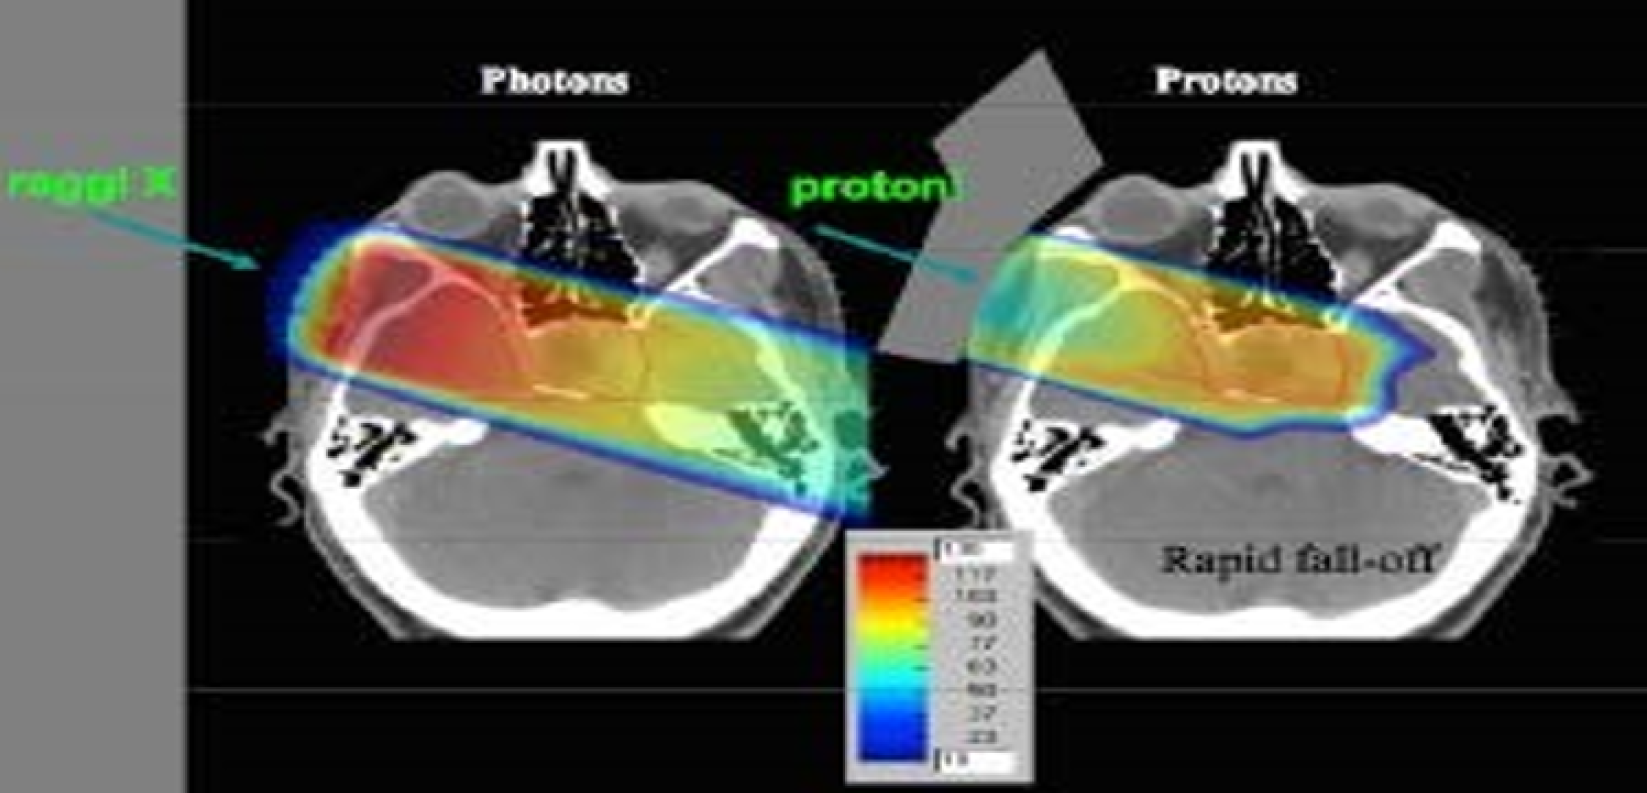
\includegraphics[width=0.7\linewidth]{IMG/ch1/Dose}
	\caption{Example of a dose distribution for a photon beam on the left and for a proton beam on the right}
	\label{fig:Dose}
\end{figure}

\noindent The energy released by the charged particles can cause both direct and indirect effects.
The direct ones are the interactions between the radiation and the biological molecules; this generates breaking points in the nucleotide chain of the DNA.
The indirect effects are the interactions, with production of free radicals, between radiations and water molecules inside the cell.
After that the free radicals interact with the biological molecules producing chemical alterations that can generate the inactivation of the cell cycle.
Damage to DNA molecules is considered the most important since it can lead to the cell's inability to reproduce and cell death\cite{cells}.
\newline
Irradiation can produce various types of alterations in the DNA structure:
\begin{itemize}
	\item \textbf{Single Strand Break} (SSB) when the nucleotide is damaged on a single DNA filament.
	\item \textbf{Double Strand Break} (DSB) when two or more nucleotide are damaged on both DNA filaments. 
\end{itemize}
Following the damage, there are several scenarios:
\begin{itemize}
	\item \textbf{Complete repair}, a situation that occurs for the majority of minor alterations (SSB), after which the cell resumes its normal activity.
	\item \textbf{Wrong repair}, in which the cell repairs its damage but not comprehensively. This can lead to the impossibility of replication of the cell or to its death by apoptosis. In some cases the cell may be able to divide, but by passing on a genetic mutation.
	\item \textbf{Unrepairable damage}, in this scenario the cell dies within a few hours due to the release of lytic enzymes or dies on the occasion of the first mitotic division. This situation occurs mainly in the case of DSB.
\end{itemize}
The cellular response to radiation depends in a complex way on the absorbed dose. In radiobiology, the biological efficacy of a radiation dose is studied by measuring cell survival as a function of the dose irradiated on the sample. The main physical factor on which biological damage depends, for the same dose administered, is the "Linear Energy Transfer" (LET)\cite{let}:   
\begin{equation}\label{eq:let}
	LET=\frac{dE}{dx}
\end{equation}
\noindent The LTE is defined as the average ionization density along the trail of a particle and is measured in keV/$\mu m$.
Radiations with high LET have, considering fixed the absorbed dose, a greater biological effect compared to the ones with low LET.
This happens because a higher ionization density imply a greater probability of unrepairable damages, like DSB.
The biological effect of a radiation is quantified in terms of Relative Biological Efficiency (RBE), defined as the ratio between the dose required to obtain a specific effect respectively with a reference radiation and with the radiation in question.
\begin{equation}\label{eq:rbe}
	RBE=\frac{D_{ref}}{D_{test}}
\end{equation}
\noindent The reference radiation $D_{ref}$ is commonly represented by a 250 keV X-ray beam, while $D_{test}$ corresponds to the dose of the radiation under examination.
\begin{figure}[H]
	\centering
	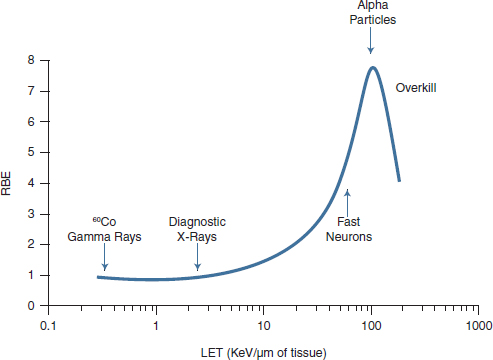
\includegraphics[width=0.7\linewidth]{IMG/ch1/RBE}
	\caption{RBE in function of the LET}
	\label{fig:rbe}
\end{figure}
\noindent In figure \ref{fig:rbe} it can be seen how the RBE changes i function of the radiation LET. From the graph it can be noted that the RBE growth, in function of the LET, starts for values near 1 keV/$\mu m$ and reaches a maximum near 100 keV/$\mu m$. For even higher LET values the RBE decreases, this is caused by a biological saturation effect that happens for high dose (overkill). 
10 MeV carbon ions have a LET of 170 keV/$\mu m$, this correspond to a RBE of 7. This is one of the reasons why therapies based on the use of carbon ions have been developed, which at the same dose, produce greater biological effects and are more effective in the treatment of radio-resistant tumors.


\section{Dose distribution systems in hadron therapy}
The physical and biological advantages of therapies with charged particles described in the previous paragraphs allow to obtain a precise conformation of the dose to the tumor, while minimizing the risk of side effects due to the irradiation of surrounding healthy organs.
These advantages are nowadays exploited in the treatment of delicate tumors in the proximity of organs at risk, pediatric tumors where the risk of side effects must be minimal, and radio-resistant tumors.
The number of patients treated with protons or carbon ions is growing each year as it can be seen in figure \ref{fig:patientstreated}
\begin{figure}[H]
	\centering
	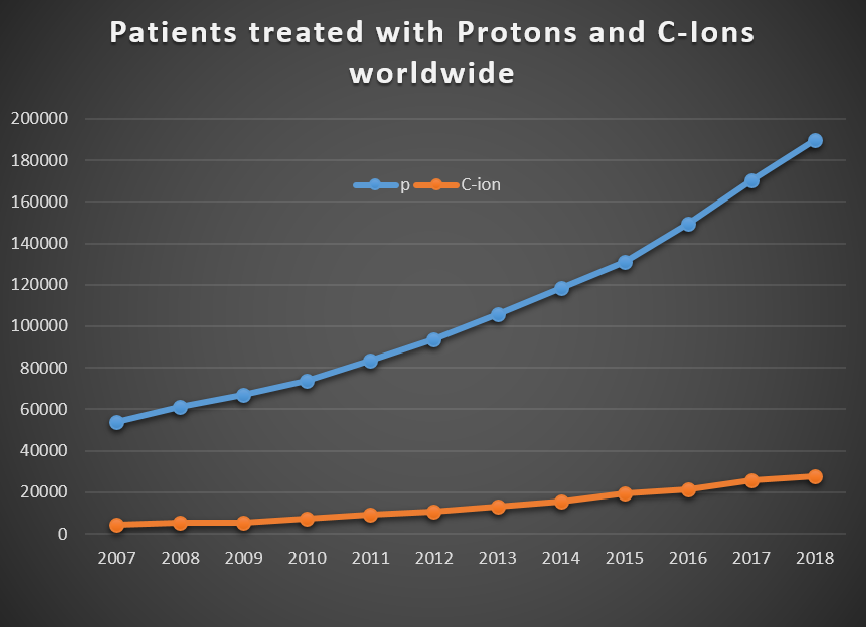
\includegraphics[width=0.7\linewidth]{IMG/ch1/PatientsTreated}
	\caption{Number of patients treated with annually with protons and carbon ions}
	\label{fig:patientstreated}
\end{figure}
\noindent This numbers, even if are growing, are still a small fraction of the total number of tumors treated with external radiation; X-ray being the main therapy method. 
The main reason lies in the need for complex accelerators (cyclotrons or synchrotrons) fundamental to accelerate the ions to
the energies needed to penetrate deeply into the tissues and a sophisticated dose distribution system that guarantees the achievable precision in delivering the dose in the various regions of the patient.
Charged particles beams used id hadron therapy are accelerated by synchrotrons or cyclotrons.
\newline
Cyclotrons take up less space and are cheaper to build and to maintain, however the accelerated particles have fixed energy that can not be changed. It can only be reduced using absorbent elements called range shifter.
On the contrary, a synchrotron can accelerate ions at different energies, but it need much more space and money to operate.
Typically a medical purpose synchrotron like the one in figure \ref{fig:sincrotrone} has a ring of at least 10m in diameter and needs one or two linear accelerators in series.
\begin{figure}[H]
	\centering
	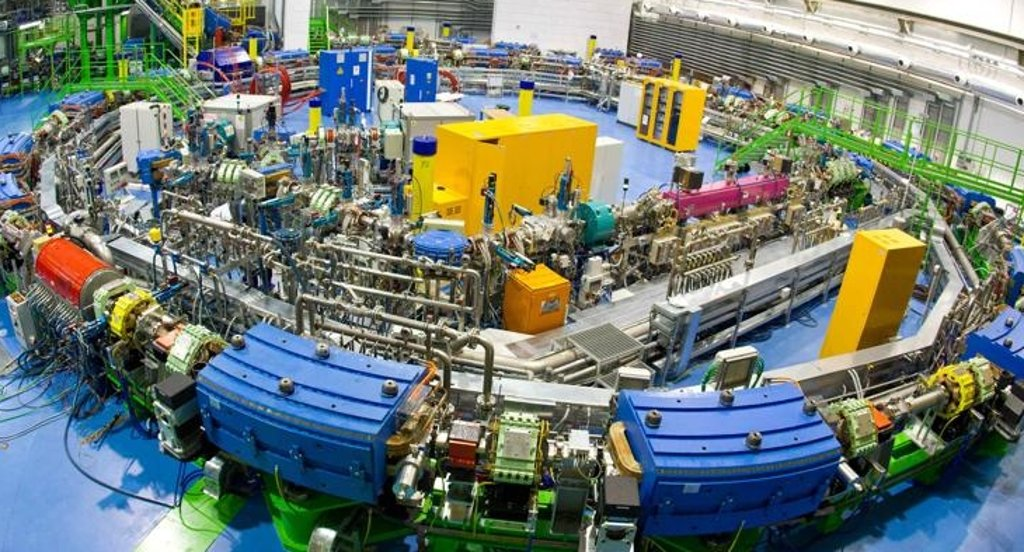
\includegraphics[width=0.7\linewidth]{IMG/ch1/Sincrotrone}
	\caption{The synchrotron at the National Center of Oncological Hadrotherapy (CNAO) of Pavia}
	\label{fig:sincrotrone}
\end{figure}
\noindent Regardless of the type of acceleration used, it is crucial that the beam remain modulated in energy and direction in such a way to produce an optimal dose distribution. This is generally achieved by producing a Spread Out Bragg Peak (SOBP), a constant longitudinal dose distribution in the volume to be treated obtained by superimposing beams at different energies, as shown in figure \ref{fig:sobp}.
\begin{figure}[H]
	\centering
	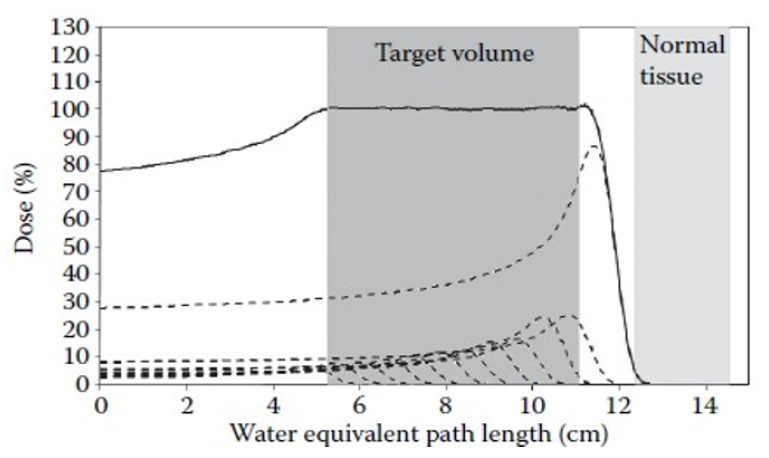
\includegraphics[width=0.7\linewidth]{IMG/ch1/SOBP}
	\caption{The SOBP is obtained by superimposing multiple beams with different energy, thus creating a dose profile constant with the depth of the tissue}
	\label{fig:sobp}
\end{figure}
\noindent There are two ways to conform the particle beam to the volume to be treated, these are passive and active distribution systems.

\subsection{Passive dose distribution systems}
\noindent Passive dose distribution techniques are mainly employed in centers where a cyclotron is used, which provides a fixed energy beam.
The passive methods consist in the use of appropriate absorbing and collimating elements that cause a broadening of the beam, modify its energy in order to produce an appropriate SOBP and adapt the lateral shape to the volume to be treated.
\begin{figure}[H]
	\centering
	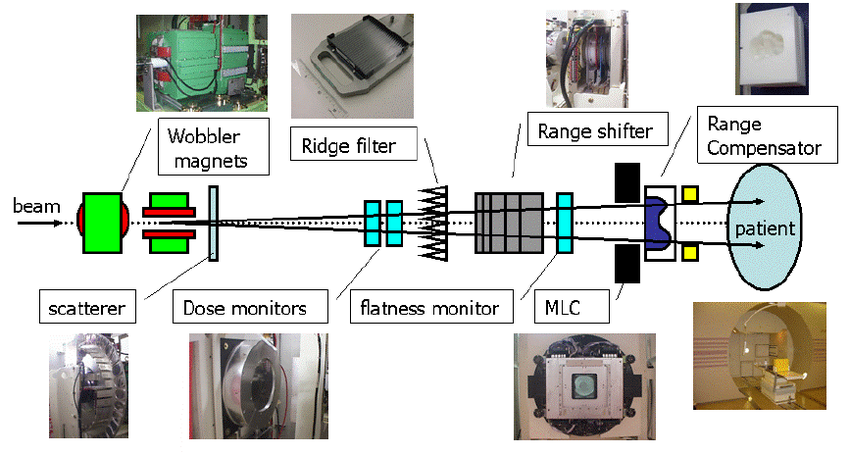
\includegraphics[width=0.7\linewidth]{IMG/ch1/Basic-design-of-irradiation-system-for-hadron-therapy}
	\caption{Basic design of passive dose distribution system for hadron therapy used to adapt the dose to the form of the tumor}
	\label{fig:passive}
\end{figure}
\noindent A typical example of passive dose distribution system is shown in figure \ref{fig:passive}. A fixed energy beam passes through a first thin layer of scattering material (scatter), like lead, that causes the beam to broaden with a simil-gaussian transverse distribution.
The thin thickness of the material means that the energy loss is minimum.
The dose is monitored with some ionization chambers.
The maximum energy and thus the SOBP is set with the use of range shifters.
The beam lateral profile is adapted to the form of the tumor with the use of collimators.
The dose is set in accordance with the shape of the tumor with the use of range compensators.
\newline
The advantages of this technique are the simplicity, safety, wide diffusion in existential hadrontherapy centers and low sensitivity to the temporal dynamics of the beam. 
On the other hand there is the reduced flexibility in the three dimensional conformation of the dose, the need to use customized collimators, the difficulty of obtaining a truly parallel beam, the low efficiency of use of the beam and the contamination of the patient due to the production of secondary fragments (for example neutrons) in nuclear interactions with absorbent elements.

\subsection{Active dose distribution systems}
\noindent Unlike passive systems in which the beam is spread to cover the entire tumor area, in active distribution systems the tumor volume is divided into a grid of points, called spots, that are grouped into several mono-energetic layers, where each layer corresponds to the position of the Bragg peak of fixed energy beam, called pencil beam.
The lateral conformation is obtained with a magnetic deflection, while the energy of the beam is changed to move the Bragg peak from one layer to the other.
In active systems based on cyclotrons, the energy of the beam is changed using absorbent materials (range shifters) of appropriate thickness, while in synchrotron-based centers, directly changing the energy at which the beam is accelerated between one spill and the next.
Scanning in the direction orthogonal to the beam is performed with two perpendicular magnets.
\newline
There are two modes of active distribution: in one the beam is moved continuously along the scanning lines and the transverse dose distribution is modulated by adjusting the scanning speed (raster scanning). A second mode (spot scanning)\cite{cnao} consists in keeping the beam fixed on a spot until the predetermined dose is reached, and then moving it, without turning it off, to the adjacent spot until the whole mono-energetic slice is is completely irradiated, as shown in figure \ref{fig:active}.
\begin{figure}[H]
	\centering
	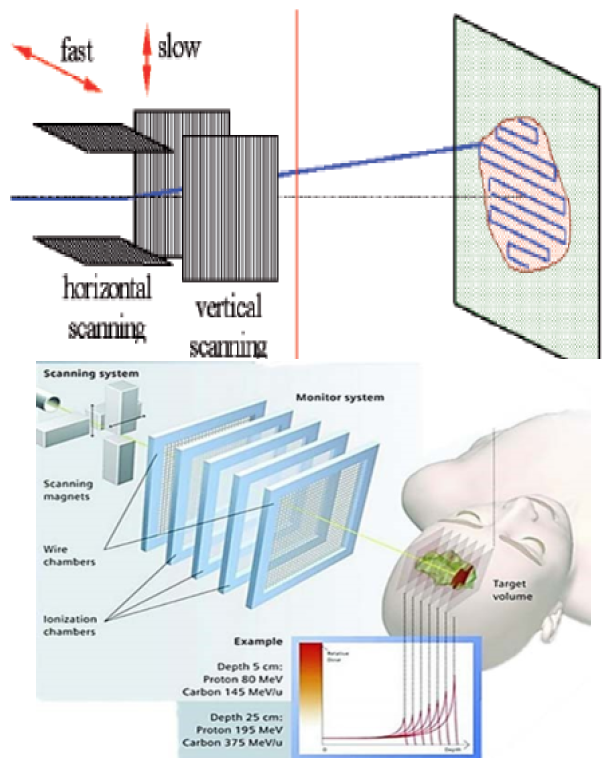
\includegraphics[width=0.7\linewidth]{IMG/ch1/Active}
	\caption{Basic design of active dose distribution system for hadron therapy used to adapt the dose to the form of the tumor. Modulated dose distribution in the transverse plane by scanning magnets (top) and on the longitudinal axis with the superposition of energy beams different (bottom)}
	\label{fig:active}
\end{figure}
\noindent This last technique provides the enormous advantage of being able to perform an extremely precise and homogeneous irradiation that adapts to the shape of the tumor which is in most cases irregular.
Another advantage compared to passive systems is the absence of material on the beam line, a lower lateral penumbra due to the absence of collimators, a high efficiency of use of the beam and the possibility to synchronize the radiation with the respiratory phase of the patient.

\subsection{Treatment Planning System}
\noindent The Treatment Planning System (TPS) is software that simulates patient dose distribution and calculates the optimal beam configuration to achieve clinical dose specifications for the tumor and healthy organs.
It is a complex tool, which uses information on the patient's anatomy as input provided by computed tomography (CT) images, with physician-designated contours of the tumor and surrounding organs.
Based on this information and the specifications of the desired target dose and the maximum tolerable dose on other organs, the TPS performs a minimization procedure (called "reverse planning") to determine the treatment parameters.
The output of the TPS provides the parameters corresponding to the number of particles, energies and directions of the pencil beam for each spot necessary to best meet the specifications.
The TPS searches for the solution iteratively: starting from an initial hypothesis on the number of particles for each spot, the program calculates the spectra of the particles for each point of interest and estimates the corresponding biological effect.
If the result meets the specifications, the TPS can terminate the execution and if not, the program must appropriately vary the number of irradiated particles and repeat the biological effect assessment, until the specifications are met or the maximum number of iterations is reached.


\section{Beam monitoring}
\noindent The accuracy of the dose distribution obtained with the active pencil beam scanning technique is based on a precise online measurement of the beam position and the number of particles irradiated at each point.
The Dose Distribution System (DDS)\cite{pencil} must control the scanning system, consisting of two power supplies connected to two orthogonal bipolar magnets to deflect the beam horizontally and vertically.
Once the required number of particles are irradiated in one spot, the DDS vary the currents in the magnets in order to move the beam to the next point.
Moreover, the DDS must be interfaced with the accelerator control to request a quick stop of the beam when a slice is completed or to request new energy values for the treatment of the next slice.
The operations of the DDS are all based on the online measurement of the number of irradiated particles and the direction of the beam carried out with dedicated detectors.
\newline
The most commonly used monitor detectors are based on ionization chambers (ICs).
Figure \ref{fig:monitor}, for example, shows the beam detector system used by the National Center of Oncological Hadrotherapy (CNAO) in Pavia, consisting of five planar ionization chambers (ICs) filled with nitrogen and positioned at the end of the beam line.
Two chambers with a single electrode provide information on the number of particles irradiated with a frequency of 1 MHz, while the other three chambers have electrodes segmented into strips or pixels for measuring the shape and position of the beam.
\begin{figure}[H]
	\centering
	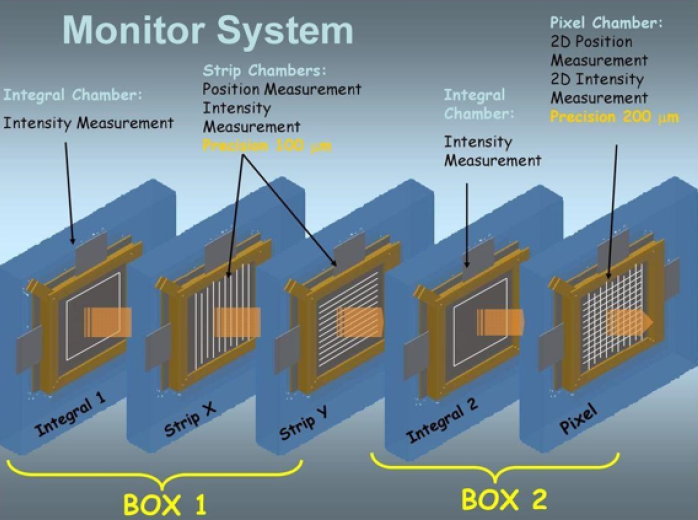
\includegraphics[width=0.7\linewidth]{IMG/ch1/MonitorSystem.PNG}
	\caption{}
	\label{fig:monitor}
\end{figure}
\noindent Due to their limited complexity, ICs offer several advantages such as robustness, ease of construction and operation, and show no indication of performance degradation due to radiation and aging effects, even after several years of operation.
Despite being the gold standard in beam monitoring applications in hadrontherapy, the imminent development of new treatment techniques are beginning to suffer from the limitations of gas detector technology.
\newline
ICs measure the charge produced in the gas, which depends not only on the number of particles, but also on the energy of the particles and environmental parameters.
To determine the number of particles irradiated on each spot, the energy of the beam must be known in advance as well as the effects of temperature and pressure dependencies must be taken into account.
Periodic calibration procedures are required to ensure the reliability of the ICs in clinical practice.
Another limitation of the ionization chambers is their limited sensitivity: due to the small ionization charge produced in gases, the minimum number of particles that an IC can detect is limited to about $10^4$ protons.
Furthermore, the collection times of the charge in the gas are relatively long (of the order of hundreds of $\mu$s) and therefore their response is rather slow.
These limitations prevent their use in treatment modalities where rapid changes in position are required or when a limited number of particles must be irradiated at each spot.
\newline
To overcome the limitations of ionization chambers as monitoring devices in hadrontherapy, as their limited sensitivity, the dependence of the measurable number of particles on the energy of the beam and environmental parameters, slow response times, the Medical Physics group of the University of Turin is studying a new approach for beam monitoring based on the solid state detector.
In particular, segmented silicon detectors are considered as an alternative to IC chambers to count the number of particles in a therapeutic beam.
\newline
In the next paragraph it is described the operation of a silicon detector, while in the next chapter it will be shown how their characteristics can compensate for the limitations of the ionization chambers.



\subsection{Silicon detectors}

\noindent Silicon is a semiconductor formed by tetravalent atoms \cite{detector}, with a resistivity between that of the metal and the insulators, with a forbidden energy band of 1.14 eV.
An electron jumping in the conduction band leaves a hole in the valence band, which behaves like a positive charge carrier.
When silicon is doped with trivalent atoms (acceptors) there is an excess of holes ("p-type" material).
Doping with pentavalent (donor) atoms produces materials with an excess of electrons (called "n-type").
\newline
A silicon detector is based on p-n junctions, and on the formation of a depletion region without free charges obtained by applying an intense reverse polarization.
In a silicon detector the depletion region is the active volume in which the hole-electron pairs are created by the ionization of the particles, similar to how ion-electron pairs are produced in a gas detector.
The current induced in the electrode during the migration of the hole-electron pairs is collected and integrated to measure the total charge produced, proportional to the loss of energy by the charged particle.
\newline
The average energy required to create a hole-electron pair is an order of magnitude smaller in silicon than in a gas (3.6 eV in Si compared to more than 30 eV in N$_2$ or in air).
Also considering the much higher density of silicon than a gas, the charge produced by an ionizing particle in a thin layer of silicon is high enough to be measurable even for a single particle.
\newline
The silicon detectors are constructed with a series of p-n junctions with the electrodes segmented into strips or pixels, and used for particle monitoring in particle physics and nuclear physics applications.
An example of a silicon strip detector is shown in figure \ref{fig:detector}. It consists of highly doped p-type strips implanted on an n-type substrate and an n ++ electrode.
The substrate n is completely emptied by applying a positive voltage on the electrode n++ with respect to the strips.
An ionizing particle penetrates the emptied substrate and generates electron-hole pairs that migrate along the electric field generated by the applied voltage and induces a current signal on the aluminum strips.
In this example, the aluminum electrodes are separated by a thin SiO2 capacitive layer (AC coupling), but configurations with direct connection of the aluminum to the n ++ electrode (DC coupling) are also possible.
\begin{figure}[H]
	\centering
	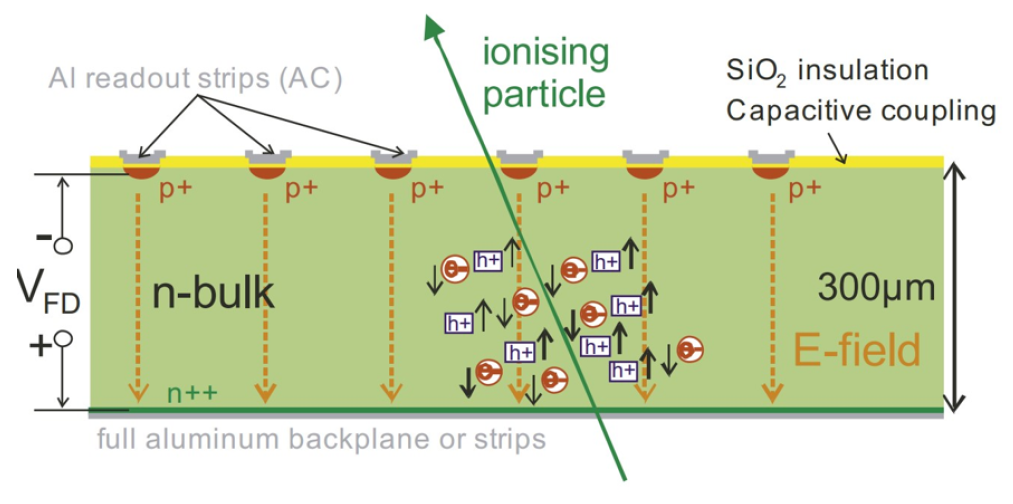
\includegraphics[width=0.7\linewidth]{IMG/ch1/Detector.PNG}
	\caption{Schematic of a silicon detector with strip segmented electrodes}
	\label{fig:detector}
\end{figure}
\noindent In a typical strip detector, the thickness of the emptying region is about 300$\mu$m to produce a sufficient charge detectable by the reading electronics. 
The typical collection time of electrons and holes varies from 3 ns to 6 ns, depending on the applied voltage.
















































	
	\chapter{Development of a device for direct counting of the number of beam particles}

\section{Introduction}
This chapter will focus on the devices under development within the MoVe\_IT project in order to obtain a single proton counting device.
This comprehends a solid state detector, the ASICs used to digitalise the signal and the final read-out board.
\begin{figure}[H]
	\centering
	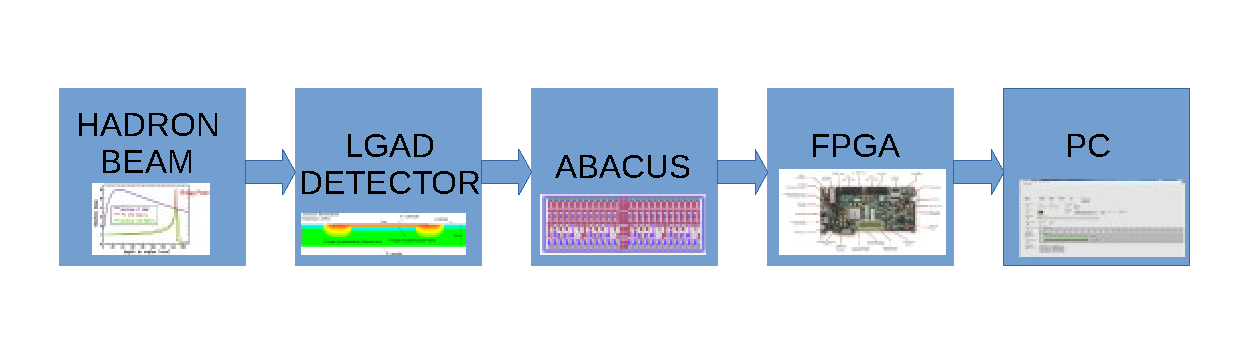
\includegraphics[width=0.99\linewidth]{IMG/ch2/BLOCK}
	\caption{Data flow, from beam to pc}
	\label{fig:block}
\end{figure}
\noindent In figure \ref{fig:block} it can be seen a diagram with the "data flow" of the Project.
The particle beam coming from the accelerators are detected by a LGAD (Low Gain Avalanche Diode) sensor that will be discussed in section \ref{lgad}, the current signal coming from the detector is the digitalized by the second version of a full custom circuit called ABACUS\_v2 that will be discussed in section \ref{chip}.
This ASIC will be mounted on a full custom PCB named EsaAbacus that will be analysed in section \ref{esaabacus}.
The data from the chip is then read by an FPGA board, a general purpose device that will be described in detail within chapter 3.
The FPGA elaborates the data and finally sends them to a computer. In the final operational device the computer, on the base of the counted particles, should move and control the beam in a close and controlled loop. 

\section{MoVe\_IT project}\label{moveit}
\begin{figure}[H]
	\centering
	
\includegraphics[width=0.35\linewidth]{IMG/ch2/Move_IT_logo}
	%\caption{}
	%\label{fig:moveit}
\end{figure}
\noindent Currently the Medical Physics group at University of Torino and INFN (the Italian National Institute for
Nuclear and Particle Physics) is participating to the MoVe\_IT\cite{moveit} (Modeling and Verification for Ion beam Treatment planning)
research project, which aims to develop new and
innovative models for biologically optimized Treatment Planning Systems (TPS) using ion beams in hadron therapy.
As~part of the project the Torino group is involved in the development of solid state detectors and readout electronics for measuring with high precision
the characteristics of the hadron beam for irradiation, such as number of particles delivered per unit time, energy and beam profile.
The final goal is to prove the ability of LGAD detectors to discriminate individual protons and to count their number up to fluxes of 100~MHz/cm$^2$ with an uncertainty of less than 1\% which is the clinical tolerance required.
In order to do that a custom detector was built ad hoc for this purpose. It is a LGAD type sensor with an area of $\approx$ 3x3~cm$^2$ and 144 strips. It has a thickness of the active region of 50~$\mu$m.
The final goal is to use two of this sensors in orthogonal directions in order to obtain a precise information on the beam position and profile.
A strip detector is limited in the maximum flux that can be monitored with accuracy, however it is useful in radiobiological experiments, for which it is not needed to reach therapeutic fluxes and often laterally spread-out beams are used\cite{hammad}.
The main key-points of the final design are:
\begin{itemize}
	\item A cover area of $\approx$ 3x3~cm$^2$
	\item A maximum measurable flux of 10$^8$~$\frac{p}{s \cdot cm^2}$ with less than 1\% error
	\item Sensitivity of single particle at low fluxes
	\item Provide beam shape in two orthogonal directions
\end{itemize}


\section{Low Gain Avalanche Diode (LGAD)}\label{lgad}
\noindent The first device involved is the detector. In order to be able to detect a single particle and to reduce the pile-up effects short signals are mandatory. To obtain a short signal the active region of the sensor needs to be the as thin as possible. However the thinner the detector the lower is the SNR (Signal to Noise Ratio).
To solve this problem it was decided to use a new type of sensors known as LGAD.
\noindent Low-Gain Avalanche Detectors (LGADs) are innovative detectors developed in collaboration with the Fondazione Bruno Kessler (FBK, Trento) which feature a moderate ($\approx$10) internal charge multiplication achieved through an additional p+ doping layer few microns depth. The increased signal-to-noise ratio allows designing very thin Ultra Fast Silicon Detectors (UFSD) designed for fast signal collection times, high rates and very good time resolution\cite{lgad}.
%%%%%%%%%%%%%%%%%%%%%%%%%%%%%%%%%%%%%%%%%%%%%%%%%%%%%%%%%%%%%%%%%%%%%%%%%%%%%%%%%%%%%%%%%%%%%%%%%%%%%%%%%%%%%%%%%
The basic doping profiles of the LGAD structure, based on a standard PIN detector, is shown in
figure \ref{fig:ufsdlgad}, showing a n++/p+/p/p++ structure.
The figure shows a highly doped n++ cathode electrode with a moderately doped p+ type region
below, known as the multiplication implant. The n-type electrode has a peak doping concentration
of order 1 $\cdot$ 10$^{19}$ cm$^{-3}$ and has a shallow profile into the bulk of $\approx$ 1 $\mu$m.
The p-type multiplication implant has a peak doping concentration of order 1 $\cdot$ 10$^{16}$ cm$^{-3}$
and has a significantly deeper profile into the bulk ($\approx$ 4 $\mu$m) than the n++ electrode. The bulk
material is high resistivity p-type silicon (approximately 10 k$\Omega$/cm) with a p++ anode electrode
on the backside.
\begin{figure}[H]
	\centering
	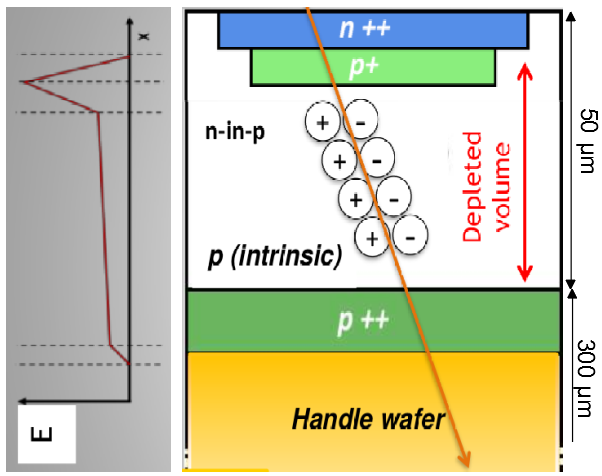
\includegraphics[width=0.35\linewidth]{IMG/ch2/UFSDLGAD.png}
	\caption{Schematic cross-section of the LGAD pad design. A p+ type layer is diffused below the n++ electrode to form the n++/p+/p junction where the multiplication takes place}
	\label{fig:ufsdlgad}
\end{figure}
\noindent The LGAD device is operated with the bulk fully depleted. Incident radiation produces electron-hole
pairs in the detector which drift towards the cathode and anode respectively. The maximum
electric field in the device is in the junction formed between the n++ cathode and the p+ type multiplication layer and is
proportional to the square root of the p+ type doping density and proportional to the square root of the
external bias voltage for an abrupt junction approximation.
The radiation induced electrons in the detector cross this high field region. For sufficiently
high electric fields impact ionisation occurs which results in multiplication of the carriers and a
signal gain.
Increasing the high-field (either due to an increase in the doping density or
an increase in the external bias voltage) will increase the electron-hole pair generation rate. For a
low gain device, the desire is to have an overall gain of 10 at $\approx$~200~V bias, with a breakdown voltage
significantly higher than this at least $\approx$~400~V.
%%%%%%%%%%%%%%%%%%%%%%%%%%%%%%%%%%%%%%%%%%%%%%%%%%%%%%%%%%%%%%%%%%%%%%%%%%%%%%%%%%%%%%%%%%%%%%%%%%%%%%%%%%%%%%%%%
\begin{figure}[H]
	\centering
	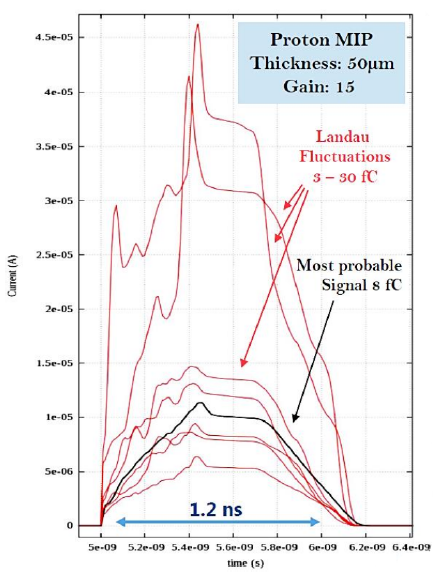
\includegraphics[width=0.35\linewidth]{IMG/ch2/LGAD_Signal}
	\caption{Simulated detector signal}
	\label{fig:signal}
\end{figure}
\noindent The output signal from a detector used in the project has a trapezoidal form, a duration of $\approx$ 1.2~ns (rise and fall times of $\approx$~450~ps and a 
flat region of $\approx$~300~ps) and a current in the order of 1$\cdot$10$^{-5}$~A.
In figure \ref{fig:signal} it can be seen a signal simulation, the most probable signal carry a 8~fC charge, however due to the Landau Fluctuations this value can change between 3~fC and 30~fC.
%%%%%%%%%%%%%%%%%%%%%%%%%%%%%%%%%%%%%%%%%%%%%%%%%%%%%%%%%%%%%%%%%%%%%%%%%%%%%%%%%%%%%%%%%%%%%%%%%%%%%%%%%%%%%%%%%
\noindent The main risk in
the use of LGAD silicon detectors for beam monitoring is related to the high radiation doses from
therapeutic beams. The design of LGAD sensors was optimized for radiation
resistance, and the measurements performed up to now indicate a stable behavior up to 10$^{15}$~n$_{eq}$/cm$^2$ for 50~$\mu$m thick detectors
(this corresponds to a few days of continous irradiation of a therapeutical proton pencil beam);
in general the internal gain
of the sensors decreases with the dose, but this can be compensated by raising the bias voltage.
%It is expected that the use of thinner sensors (50~$\mu$m thickness) will decrease the trapping
%probability in the sensors, therefore extending the operative time. Intense work is currently going
%on in the LGAD community to increase the radiation resistance of the sensors. Several
%approaches as alternative dopants and doping profiles are being investigated with the expectation
%to reach a stable behavior up to >1015~n$_{eq}$/cm$^2$ fluencies in the next 1 or 2 years.


\section{ABACUS\_v2 chip}\label{chip}
\noindent The signal from each detector strip, that can be seen in figure \ref{fig:signal}, is connected to an input channel of the new ABACUS\_v2 full custom chip\cite{abacus}\cite{dac} designed by the Turin INFN group and submitted on October 26$^{th}$ 2020.
\begin{figure}[H]
	\centering
	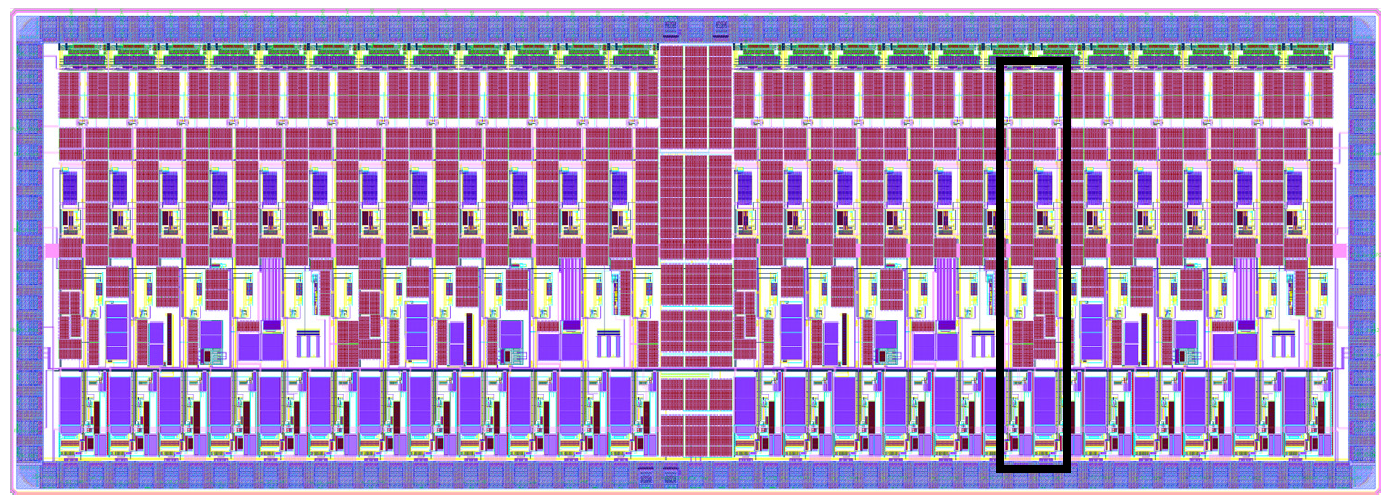
\includegraphics[width=0.9\linewidth]{IMG/ch2/ABACUS2.png}
	\caption{ABACUS\_v2 chip die view}
	\label{fig:abacus2}
\end{figure}
\noindent In figure \ref{fig:abacus2} it can be seen a schematic of the chip die area. Inside the black rectangle it can be seen a single channel. Its design will be analysed later in this section.
This prototype is a 24 channels ASIC designed in UMC (United Microelectronics Corporation) 110~nm technology.
The die size is 4.95~x~1.935~mm$^2$.
The 24 channels are divided in two 12-channels groups. The two groups differs for the architecture of the first stage only.
The first group (group A) is based on a TIA (Trans-Impedance Amplifier) architecture with a two stage core amplifier.
The second group (group B) is based on a Regulated Common Gate (RCG) input stage followed by a single stage TIA.
The pro and cons of the two architectures will not be a part of this thesis.\\
As already discussed, the design goal of the counting device is to measure the number of protons with a maximum error of 1\% up to a fluxes of 10$^8$~p/(cm$^2$$\cdot$s).
For a single particle the efficiency must be greater than 99\%, and this defines the range of charges the electronics must be able to accept.
The ABACUS\_v2 chip was optimized for an input capacitance between 5 and 20 pF and to cope with continuous signals up to 100 MHz rate.
It can accept input charges from 3~fC to 140~fC, has a dead time <~10~ns and a SNR~>~10. 

\subsection{ABACUS\_v2 Channel structure}
In order to understand the measurements from chapter 5 and the goal of this thesis work it is extremely important to analyse how the ABACUS\_v2 channel works.
In figure \ref{fig:abacuschannel} the block diagram of one channel is shown.
\begin{figure}[H]
	\centering
	\includegraphics[width=0.8\linewidth]{IMG/ch2/Abacus_channel.png}
	\caption{Single channel diagram of the ABACUS\_v2 chip}
	\label{fig:abacuschannel}
\end{figure}
\noindent A low noise CSA (Charge Sensitive Amplifier) (1) is followed by a low-pass filter (2).
The output signal from (2) has two components, a DC one, that is called Pedestal, and the actual amplified signal; this will be explained with more details in section \ref{considerations}.
The amplified signal is therefore fed to a leading-edge multistage discriminator (3 and 4) followed by a driver (5 and 6) which provides a logic pulse in Current Mode Logic (CML) format.
The output of the discriminator is also used in a feedback circuit (7 and 8) to reset the CSA feedback capacitance. This feedback circuit was designed for a fast baseline restoring and to avoid signal saturation (fast-reset signal).
The chip was heavily tested by INFN expertises; the output voltage from the amplifier and the noise were estimated by the measurement of the number of detected pulses as a function of the threshold value. The results, in terms of amplifier otutput voltage ad a function of the input charge, are shown in figure \ref{fig:abacustest} for charges between 3 fC and 20 fC\cite{abacus}.
\begin{figure}[H]
	\centering
	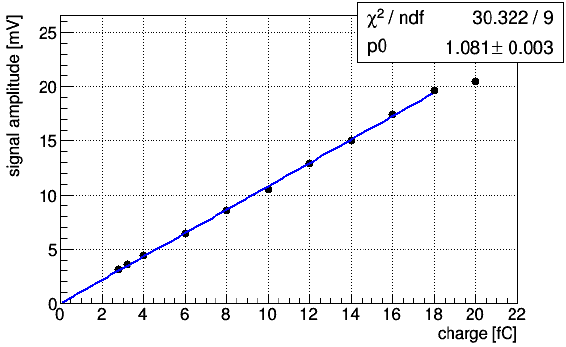
\includegraphics[width=0.6\linewidth]{IMG/ch2/ABACUSTEST}
	\caption{Amplitude of the amplifier output signal as a function of the charge injected at 1 MHz rate}
	\label{fig:abacustest}
\end{figure}
\noindent The most important considerations concern the functioning of the discriminator (3).
The threshold voltage (V$_{th}$) is the sum of two different components that are independently configurable:
\begin{itemize}
	\item An external 16~bit DAC (Digital to Analog Converter) for the global V$_{th}$ 
	\item A programmable 6~bit internal DAC for threshold tuning for each individual channel
\end{itemize}
\noindent The main external DAC provides the same threshold voltage for every channel, however due to manufacturing tolerances not every channel behaves in the same way. One may have a slightly higher or lower input capacitance, or the amplifier could have a extremely low, but measurable, difference in gain or in the baseline.    
These inequalities may have a relevant impact on the measured particle rate.
In order to reduce these differences each channel has an independently programmable 6~bit DAC that is used to fine-tune (trim) the V$_{th}$ value.    
\subsubsection{External DAC}
The external DAC is a commercially available Linear Technology LTC2604 Quad 16-bit Rail-to-Rail DAC.
The device uses the $I^2C$ protocol and reads 24~bit words configured as in figure \ref{fig:extdactiming2}; more details are provided in the data-sheet \cite{LTC2604}.
The main features are:
\begin{itemize}
	\item A guaranteed 16~Bit Monotonic Over Temperature
	\item An ultra-low Cross-talk Between DACs (<~5~$\mu$V)
	\item Separate Reference Inputs for each DAC
	\item Wide 2.5~V to 5.5~V Supply Range
	\item Low Power Operation: 250~$\mu$A per DAC at 3~V
\end{itemize} 
\begin{figure}[H]
	\centering
	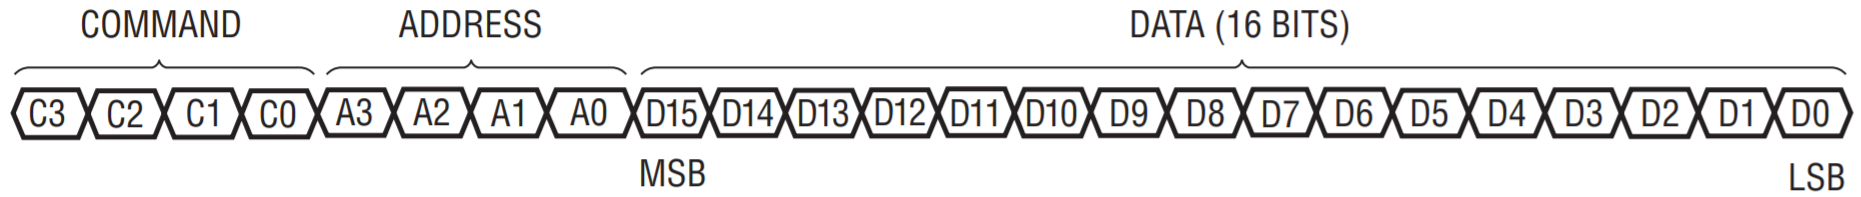
\includegraphics[width=0.99\linewidth]{IMG/ch2/EXTDACTIMING2}
	\caption{24~bit data sequence for the LTC2604 external DAC}
	\label{fig:extdactiming2}
\end{figure}
\subsubsection{Internal (Trimming) DAC}
The internal (Trimming) DACs, also called Baseline DACs, were designed specifically for this chip. Inside the die there is an $I^2C$ controller used to enable the communication between DAC and the external world.
The DACs are programmed using 16~bit serial words; the configuration process is explained in detail in section \ref{InternalDac}.
\begin{figure}[H]
	\centering
	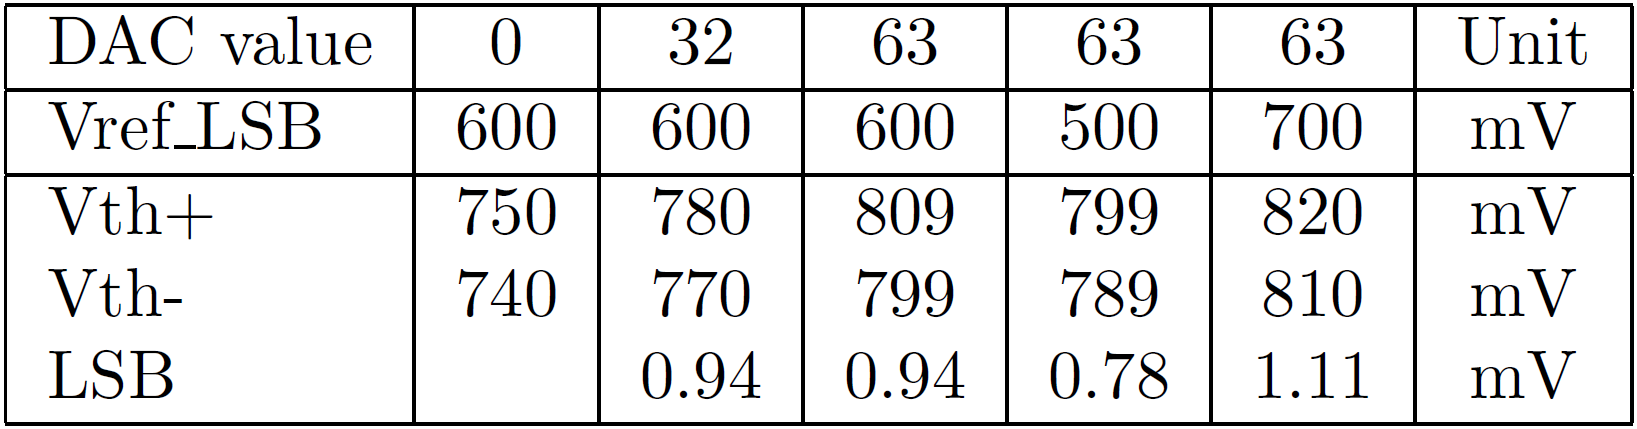
\includegraphics[width=0.5\linewidth]{IMG/ch2/INTDACTABLE}
	\caption{Internal DACs LSB values at different V$_{refLSB}$ settings}
	\label{fig:intdactable}
\end{figure}
\noindent In figure \ref{fig:intdactable} it can be seen that with a reference voltage of 600~mV the LSB should be 0.94~mV, this means that, being this a 6~bit DAC, the maximum trimming voltage is $\approx$~59.2~mV. For reference, an usual value for the pedestal voltage in around $\approx$~560~mV. Thus these internal DACs are used to fine tune the threshold voltage of the discriminator, while the bulk of the work is done by the external one.   
\newpage
\section{ESA-ABACUS}\label{esaabacus}
\noindent As explained in section \ref{moveit} the final detector will have 144 strips, however each ABACUS\_v2 chip can read only 24 channels; this means that for the ultimate sensor read-out 6 chips are needed (24$\cdot$6~=~144).
In order to utilize these device at the same time the Turin INFN group developed, built and tested a new board, called ESA-ABACUS, that can accommodate and handle 6 ABACUS\_v2 chips. The ESA-ABACUS board can be seen in figure \ref{fig:esaabacus}.
\begin{figure}[H]
	\centering
	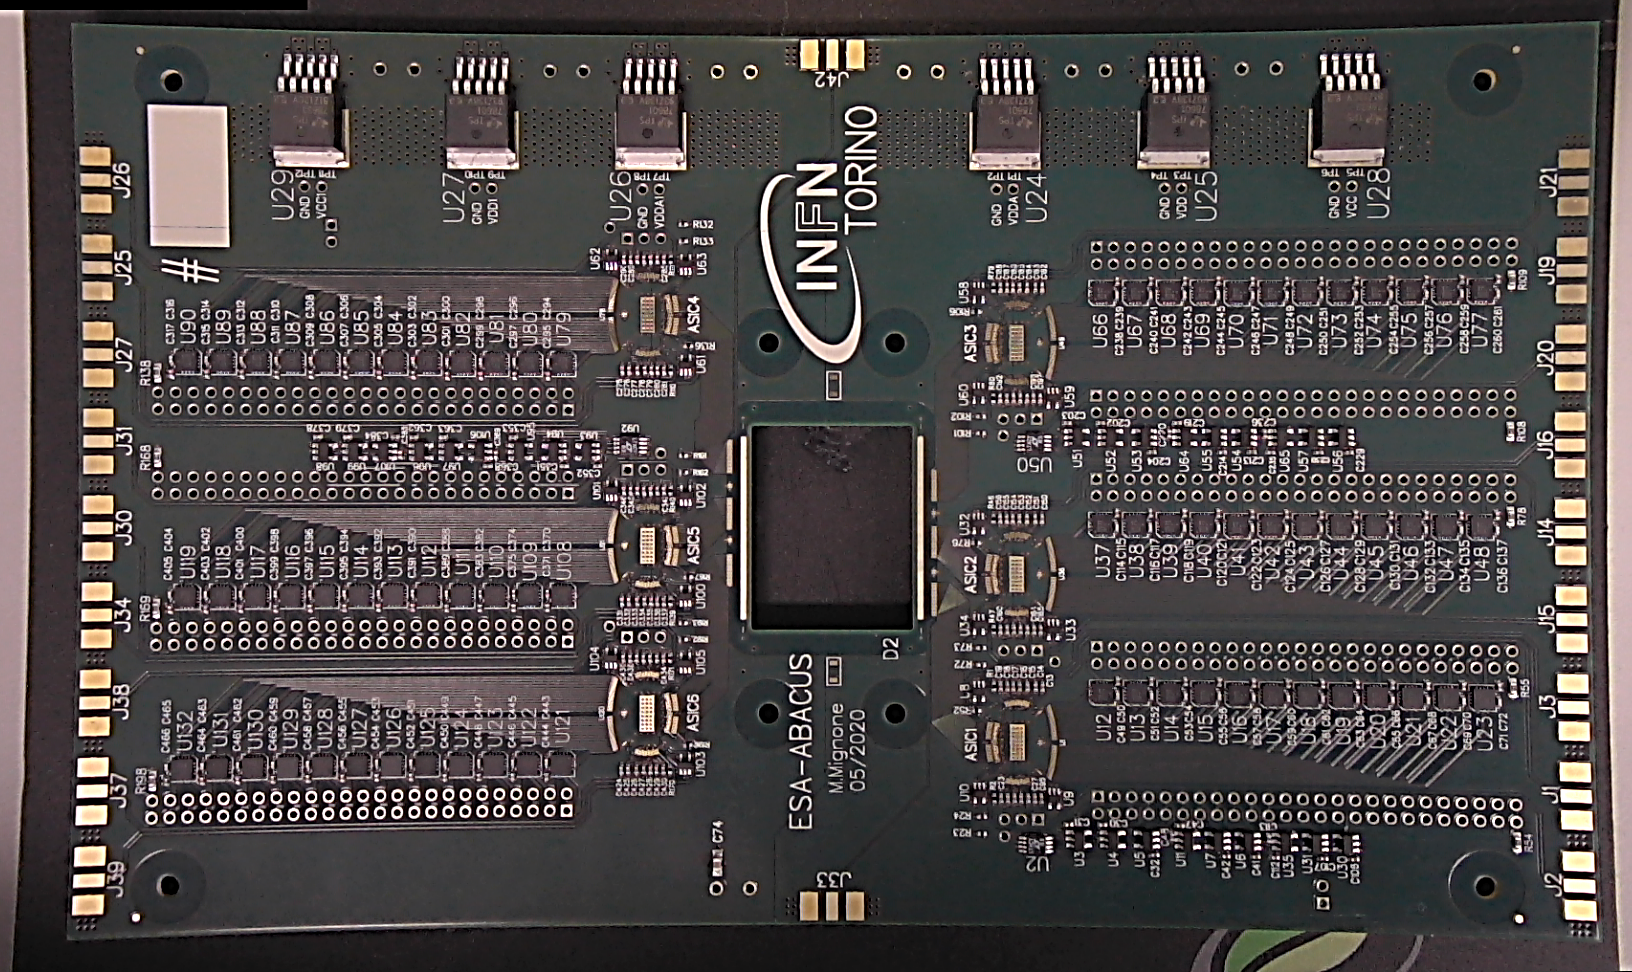
\includegraphics[width=0.7\linewidth]{IMG/ch2/EsaAbacus.png}
	\caption{Esa-Abacus board, chips and detector are not yet bonded}
	\label{fig:esaabacus}
\end{figure}
\noindent To be noted that each FPGA board used has enough Input/Output resources for two ABACUS\_v2 chips, this means that in order to utilize at his full potential the ESA-ABACUS three FPGA boards are needed (chapter 3 will explain in detail what an FPGA is).
The final goal is to use two of these devices placed in an orthogonal way in order to acquire the horizontal and vertical dispersion of the particle beam.
To be noted that this board, on the contrary of the ABACUS\_v2 test board that will be described in section \ref{testboard}, is not intended for the validation of the chip, in fact it has no trimmers for any voltage regulation, instead it was made in order to test and utilize the 144 strip detector.
The output signals from the ABACUS\_v2 chips use CML logic standard, however the FPGA boards used for the readout only support LVDS logic signals. In order to make the chip and FPGA communicate each ESA-ABACUS board has CML-LVDS converters installed.


\section{FPGA board tasks}
\noindent As explained in previous sections the digital data coming from the ABACUS\_v2 chip is analysed by an FPGA board. In this section it will be described what this devices is used for, which are its tasks and what I will implement in the new version of the firmware.
The FPGA (Field Programmable Gate Array, chapter 3) board, is a programmable device that allows to build complex electronic logic circuits with multiples Input/Output ports and many LUTs, RAMs and FIFOs by "just typing" the desired logic on a computer.
In this case the \textit{desired logic} does three main things: 
\begin{itemize}
	\item it de-serialize the input data from the chip with a 1~GHz sampling rate (500~MHz clock in DDR [Double Data Rate]), it counts the transitions from \textit{low} to \textit{high} using a manually written LUT (Look Up Table) and then it adds the result to a counter. This final value is the number of particles detected for a channel. The board does this process for each channel of the chip. In addition, by analysing the AND and OR logic combination serial data from two adjacent channels and using some maths it is possible to reduce the pile-up effects and extend the measurable rate range; this will be very briefly explained in section \ref{structure}.    
	\item it configures the internal (trimming) DACs (see chapter 4) and the external DAC used to set the V$_{th}$. In addition, it controls the LCD display of the board, can read the board's switches and button and it can turn on or off the board's LED. 
	\item it send the data to a computer using UDP (User Datagram Protocol) via a Ethernet (RJ45) cable.  
\end{itemize}

















	
	\chapter{FPGA: historical introduction, structure, design flow, VHDL and use in the MoVe\_IT project}
\section{Introduction}
\noindent Digital electronics is concerned with circuits which represent information using a finite set of output
states. Most of the applications use in fact just two states, which are often labelled ‘0’ and ‘1’.
Behind this choice is the fact that the whole Boolean formalism then becomes available for the
solution of logic problems, and also that arithmetic using binary representations of numbers is a very
mature field\cite{fpga1}.
\newline
In addition, having only two
different values for the voltages or currents used to represent states is the safest choice in terms of
design margins in order to protect the data from the noise.



\section{Programmable Logic Devices history}
\noindent Historically, TTL (Transistor–Transistor Logic) chips fuelled an initial wave of digital system designs in
the 1970s.
%This section will focus on the separate branches that evolved to satisfy the demand
%for programmability of different logic functions.
By programmability, it is meant the ability of a
designer to affect the logic behaviour of a chip after it has been produced in the factory.
\newline
\noindent A first improvement in the direction of programmability came with the introduction of gate
arrays, which were nothing else than a chip filled with NAND gates that the designer could
interconnect as needed to generate any logic function he desired.
This interconnection had to happen
at the chip design stage, thus before production, but it was already a convenient improvement over
designing everything from scratch. Until the introduction of Programmable Logic
Arrays (PLAs) in the 1980s no real programmable solution was available. These were two-level AND-OR
structures with user-programmable connections.
%\begin{figure}[H]
%	\centering
%	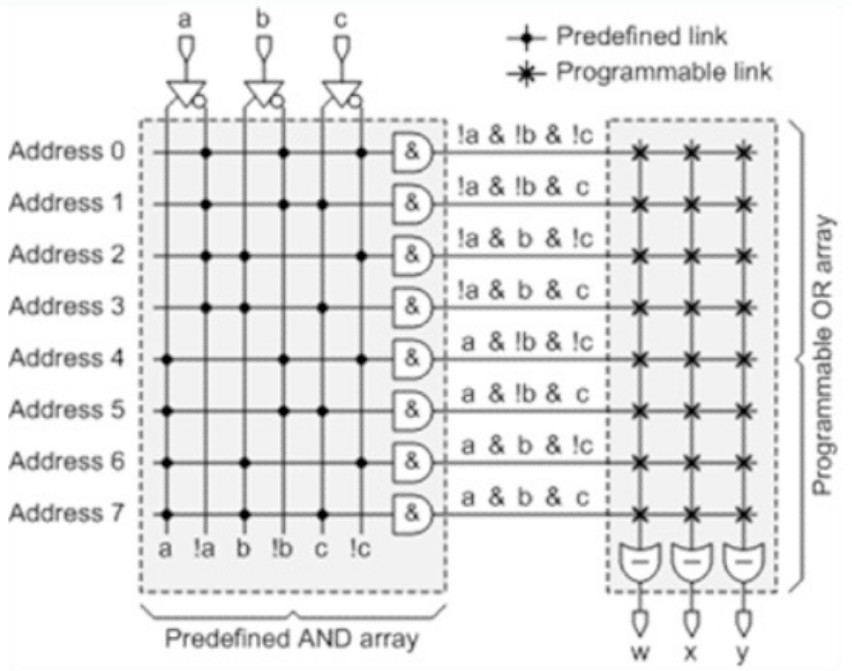
\includegraphics[width=0.7\linewidth]{IMG/ch3/PLD}
%	\caption{Unprogrammed PROM (Fixed AND Array, Programmable OR Array)}
%	\label{fig:pld}
%\end{figure}

\noindent Programmable Array Logic (PAL) devices were an
improvement in performance and cost over the PLA structure. Today, these devices are collectively
called Programmable Logic Devices (PLDs).

\noindent The next stage in sophistication resulted in Complex PLDs (CPLDs), which were nothing else
than a collection of multiple PLDs with programmable interconnections. FPGAs, in turn, contain a
much larger number of simpler blocks with the attendant increase in interconnect logic, which in fact
dominates the entire chip.
\begin{figure}[H]
	\centering
	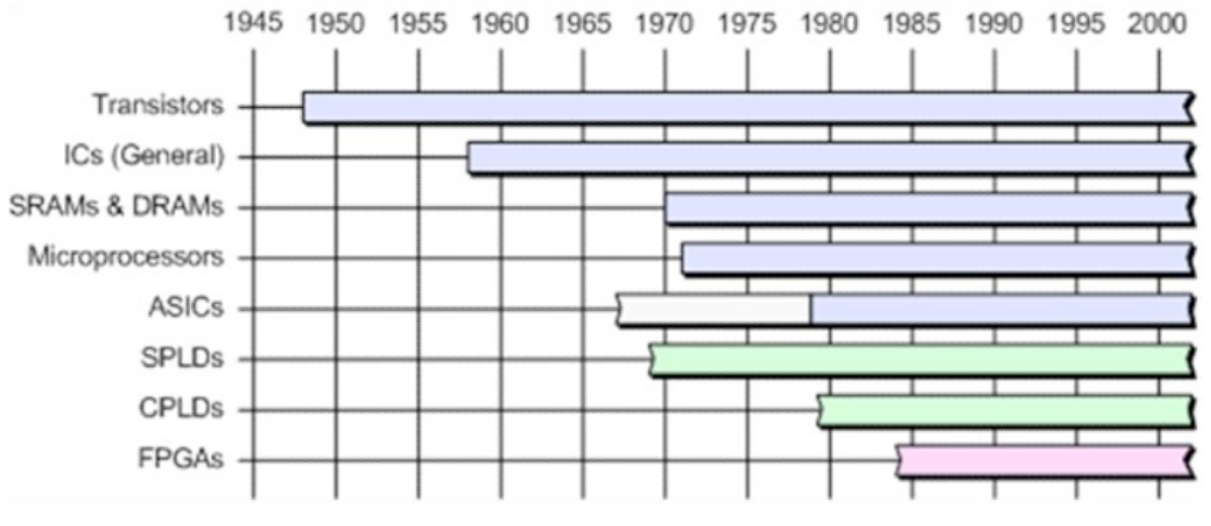
\includegraphics[width=0.7\linewidth]{IMG/ch3/TIME}
	\caption{Appearance over the years of programmable logic devices\cite{fpga3}}
	\label{fig:time}
\end{figure}
%\subsection{FPGA}
\noindent Xilinx introduced the first Field Programmable Gate Arrays
(FPGAs) in 1984, though they were not called FPGAs until
Actel popularized the term around 1988\cite{fpga2}. Since their introduction, FPGA devices have progressed
through several distinct phases of development.
Each phase was driven by both process technology opportunity
and application demand. These driving pressures
caused observable changes in the device characteristics
and tools. Each age is eight years long and each
became apparent only in retrospect. The three ages are:
\begin{itemize}
	\item Age of Invention 1984–1991
	\newline
	The first FPGA, the Xilinx XC2064, contained only 64 logic blocks, each of which held two three-input Look-Up Tables (LUTs) and one register, less than 1000 gates.
	\item Age of Expansion 1992–1999
	%\newline
	
	\item Age of Accumulation 2000–2007
	%\newline
	
\end{itemize}

\section{FPGA Versus PAL}
\noindent Programmable logic was well established before the
FPGA. EPROM-programmed Programmable Array Logic
(PAL) had carved out a market niche in the early 1980s.
However, FPGAs had an architectural advantage. To understand
the FPGA advantage, we first look at the simple
programmable logic structures of these early 1980s devices.
A PAL device, as depicted in figure \ref{fig:pal}, consists of a two level
logic structure. Inputs are shown entering at
the bottom. On the left side, a programmable and array
generates product terms, ands of any combination of the
inputs and their inverses. A fixed or gate in the block at
the right completes the combinational logic function of the
macrocell’s product terms. Every macrocell output is an
output of the chip.
\begin{figure}[H]
	\centering
	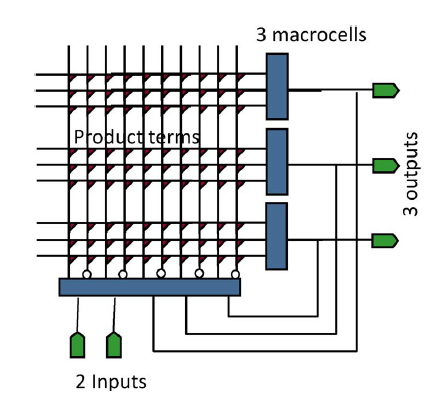
\includegraphics[width=0.7\linewidth]{IMG/ch3/PAL}
	\caption{Generic PAL architecture}
	\label{fig:pal}
\end{figure}
\noindent Nearly all common functions could be implemented in one pass through the PAL's macrocell array.
The delay through the PAL array is the same regardless of the function performed or where it is located in the array.
PALs had simple fitting software that mapped logic quickly to arbitrary locations in the array with no performance concerns.
PALs were very efficient from a manufacturing point of view.
However, the architectural issue with PALs is evident when one considers scaling. The number of programmable points in
the and array grows with the square of the number of inputs. PAL input and product-term lines are also
heavily loaded, so delay grows rapidly as size increases. To maintain speed, power consumption rose dramatically. Large PALs were
impractical in both area and performance.
\newline
The FPGA innovation was the elimination of the and array that provided the programmability. Instead, configuration
memory cells were distributed around the array to control functionality and wiring. This change gave up the
memory-array-like efficiency of the PAL structure in favor of architectural scalability. The architecture of the FPGA,
shown in figure 4, consists of an array of programmable logic blocks and interconnect with field-programmable switches.
\begin{figure}[H]
	\centering
	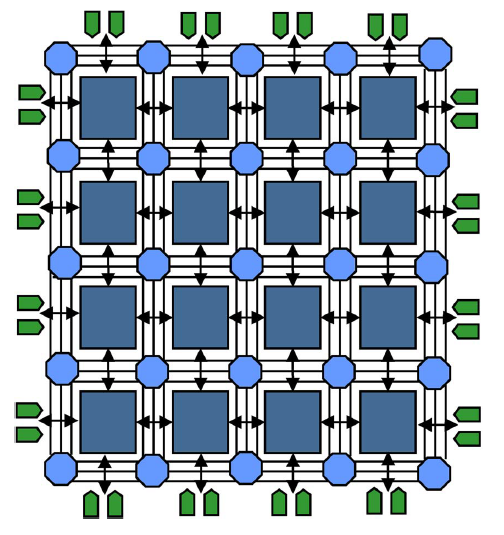
\includegraphics[width=0.7\linewidth]{IMG/ch3/FPGA}
	\caption{Generic array FPGA architecture. 4x4 array with three wiring
		tracks per row and column. Switches are at the circles at intersections.
		Device inputs and outputs are distributed around the array.}
	\label{fig:fpga}
\end{figure}
\noindent The consequences of this change were:
\begin{itemize}
	\item FPGA architecture could look nothing like a memory. Design and manufacturing were very different than memory.
	\item The logic blocks were smaller. There was no guarantee that a single function would fit into one. Therefore, it was difficult to determine ahead of time how much logic would fit into the FPGA.
	\item The performance of the FPGA depended on where the logic was placed in the FPGA. FPGAs required placement and routing, so the performance of the finished design was not easy to predict in advance.
	\item Complex EDA (Electronic Design Automation) software was required to fit a design into an FPGA.
\end{itemize}




\section{FPGA vs ASIC}
\noindent In the 1980s, Application-Specific Integrated Circuit
(ASIC) companies brought an amazing product to the
electronics market: the built-to-order custom integrated
circuit. By the mid-1980s, dozens of companies were selling
ASICs, and in the fierce competition, the winning attributes
were low cost, high capacity and high speed.When
FPGAs appeared, they compared poorly on all of these
measures, yet they thrived. The ASIC functionality was determined by custom mask
tooling. ASIC customers paid for those masks!
Because they had no custom tooling, FPGAs reduced the up-front
cost and risk of building custom digital logic. By making
one custom silicon device that could be used by hundreds or
thousands of customers, the FPGA vendor effectively
amortized the costs over all customers.
\begin{figure}[H]
	\centering
	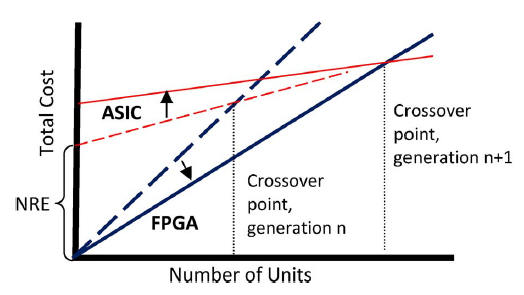
\includegraphics[width=0.7\linewidth]{IMG/ch3/COST}
	\caption{FPGA versus ASIC Crossover Point. Graph shows total cost
		versus number of units. FPGA lines are darker and start at the lower
		left corner. With the adoption of the next process node (arrows
		from the earlier node in dashed lines to later node in solid lines),
		the crossover point, indicated by the vertical dotted line, grew larger.
	\newline NRE (non-recurring engineering cost).}
	\label{fig:cost}
\end{figure}     
\noindent  An FPGA has no NRE charge, but each unit costs more than the
functionally equivalent ASIC, hence the steeper line. The
two lines meet at the crossover point. If fewer than that
number of units is required, the FPGA solution is cheaper;
more than that number of units indicates the ASIC has
lower overall cost.
\newline
Today, device cost is less of a driver in the FPGA
versus ASIC decision than performance, time-to-market,
power consumption, I/O capacity and other capabilities. Many ASIC customers use older process technology,
lowering their NRE cost, but reducing the per-chip cost
advantage. Not only did FPGAs eliminate the up-front masking
charges and reduce inventory costs, but they also reduced
design costs by eliminating whole classes of design problems.
These design problems included transistor-level design,
testing, signal integrity, crosstalk, I/O design and
clock distribution.

\section{FPGA structure}
\begin{figure}[H]
	\centering
	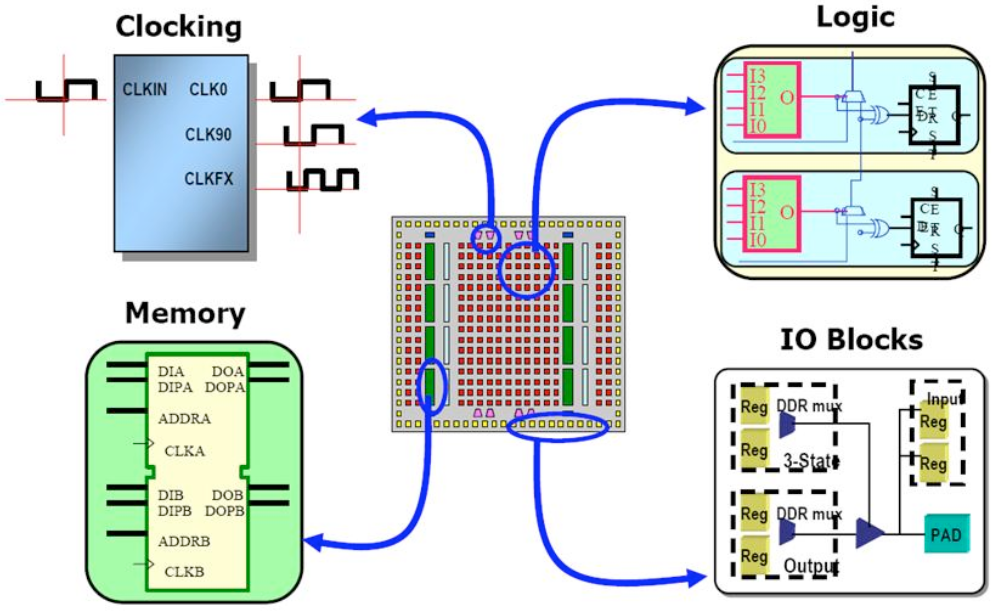
\includegraphics[width=0.7\linewidth]{IMG/ch3/FPGA2}
	\caption{Internal structure of a generic FPGA}
	\label{fig:fpga2}
\end{figure}
\noindent A typical modern FPGA, like in figure \ref{fig:fpga2}, provides the user with programmable logic blocks that
contain the pool of combinatorial blocks and flip-flops to be used in the design. In addition, vendors
acknowledge the fact that logic is often used with memory, and typically include
variable amounts of static Random Access Memory (RAM) inside their chips. Clock conditioning has
also become commonplace, and support in the form of Delay Locked Loops (DLLs) and Phase Locked
Loops (PLLs) is also provided inside the same silicon chip. Finally, an FPGA chip needs to be easily interfaced to other chips or
external signals. In order to make this interfacing easier, FPGA vendors have invested a great deal of
effort in enhancing the flexibility of the input/output blocks behind the chip pads. Each pad can serve
as an input, an output, or both. The list of electrical standards supported is extensive, and novel
techniques for maximizing bandwidth, such as clocking data in using both edges of the clock, are
widely supported.
\newline
All the components shown in figure \ref{fig:fpga2}, however, typically account for less than 20\% of the silicon
inside an FPGA chip. What is not shown is the large amounts of programmable interconnect and the
auxiliary circuits which ‘program’ the generic blocks to become a well-defined piece of logic.
To overcome the silicon inefficiency problem, FPGA vendors often include hardwired
Intellectual Property (IP) cores inside the chips for functions identified as recurrent in many designs.
These non-programmable blocks include general-purpose processors, high-speed serial interfaces,
arithmetic blocks and Ethernet Medium Access Control (MAC) units.
\\
FPGAs are truly parallel in nature so different processing operations do not have to compete for the same resources. As a result, the performance of one part of the application is not affected when additional processing is added.
\newline
\noindent In figure \ref{fig:fpga} it can be seen that the three more important blocks that made a FPGA chip are: Configurable logic Blocks (CBLs, blue squares); Input/Output Blocks (IOBs, green rectangles); Programmable Switch Matrixs (PSMs, blue octagon).
\begin{itemize}
	\item \textbf{CBLs}: Each CLB consists of n-input Lookup table and a pair of programmable flip flops. In Xilinx logic block, figure \ref{fig:clb}, a Look up table is used to implement any number of different functionality. The output of the lookup table gives the result of the logic function that it implements. Lookup table is implemented using SRAM (Static Random Access Memory).
	\begin{figure}[H]
		\centering
		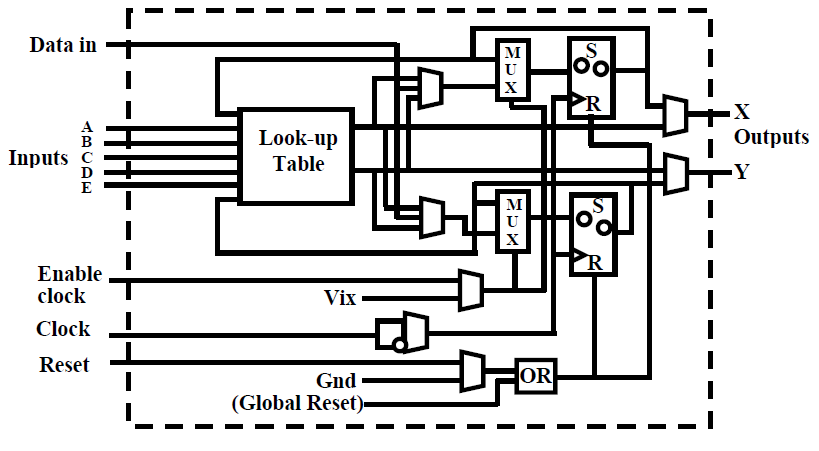
\includegraphics[width=0.7\linewidth]{IMG/ch3/CLB}
		\caption{Xilinx - LUT based configurable logic block}
		\label{fig:clb}
	\end{figure}
	\item \textbf{IOBs}: I/O blocks control functions such as tri-state buffer control, output transition speed (Slew Rate).
	\newline
	Provides to the chip a minimum of over-current and over-voltage protection and the right termination for each specific type of signalling.
	\item \textbf{PSMs}: Interconnects provide routing path. Using 6 CMOS switches controlled by a 6-bit data can be controlled a  wire intersection. Being \textbf{A}, \textbf{B}, \textbf{C} and \textbf{D} the  end of the routing the following connections can be made: \textbf{AB}, \textbf{AC}, \textbf{AD}, \textbf{BC}, \textbf{BD} and \textbf{CD}.
	\newline
	The data for each PSM is stored in a SRAM.
\end{itemize}
\noindent Thus a board its configured in two ways:
\begin{itemize}
	\item By setting the intersections (SMBs) between the logic blocks.
	\item By setting the function of each logic block.
\end{itemize}
\section{FPGA design flow and tools}
\noindent The most common flow nowadays used in the design of FPGAs involves the following
subsequent phases:
\begin{itemize}
	\item \textbf{Design entry}: This step consists in transforming the design ideas into some form of
	computerized representation. This is most commonly accomplished using Hardware Description
	Languages (HDLs). The two most popular HDLs are Verilog and the Very High Speed
	Integrated Circuit HDL (VHDL), used fot my thesis work. It should be noted that an HDL, as its name implies, is only
	a tool to describe a design that pre-existed in the mind, notes, and sketches of a designer. Another point to note is that HDLs differ from
	conventional software programming languages in the sense that they don’t support the concept
	of sequential execution of statements in the code. This is easy to understand if one considers the
	alternative schematic representation of an HDL file: what one sees in the upper part of the
	schematic cannot be said to happen before or after what one sees in the lower part.
	This is the only human-labour intensive part of the design process.
	\item \textbf{Simulation}: Typically, the design entry step is followed or interspersed with periods of functional simulation. That's where a simulator is used to execute the design and confirm that the correct outputs are produced for a given set of test inputs\cite{fpga4}. This section will be analyzed in more detail later on in this chapter.
	\item \textbf{Synthesis}: The synthesis tool receives HDL and a choice of FPGA vendor and model. From
	these two pieces of information, it generates a netlist which uses the primitives proposed by the
	vendor in order to satisfy the logic behaviour specified in the HDL files.
	\item \textbf{Place and route}: The placer takes the synthesized netlist and chooses a place for each of the
	primitives inside the chip. The router’s task is then to interconnect all these primitives together
	satisfying the timing constraints. The most obvious constraint for a design is the frequency of
	the system clock, but there are more involved constraints one can impose on a design using the
	software packages supported by the vendors.
	\item \textbf{Bit stream generation (Download)}: FPGAs are typically configured at power-up time from some sort of
	external permanent storage device, typically a flash memory. Once the place and route process is
	finished, the resulting choices for the configuration of each programmable element in the FPGA
	chip, be it logic or interconnect, must be stored in a file to program the flash.
	
\end{itemize}

\begin{figure}[H]
	\centering
	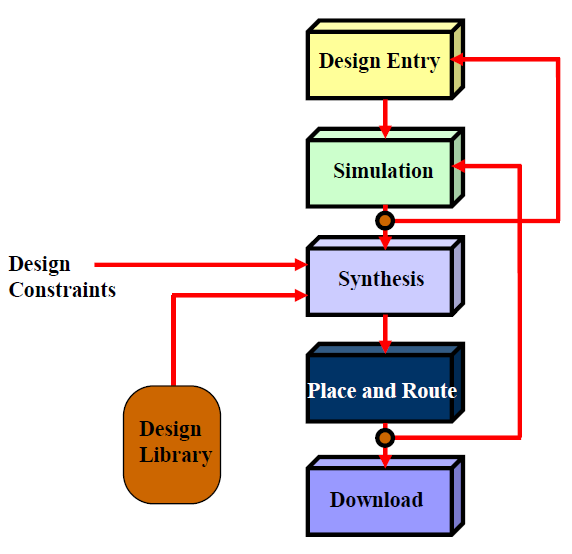
\includegraphics[width=0.7\linewidth]{IMG/ch3/FLOW}
	\caption{Programmable logic, in this case FPGA, design process}
	\label{fig:flow}
\end{figure}

\section{Hardware Description Language}
\begin{figure}[H]
	\centering
	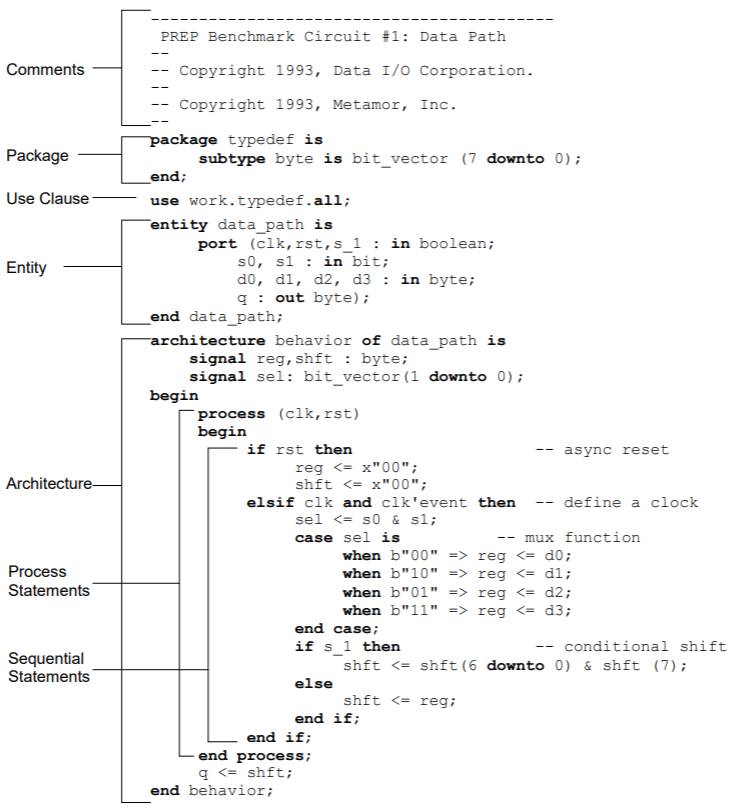
\includegraphics[width=0.7\linewidth]{IMG/ch3/VHDL}
	\caption{The structure of a VHDL design description}
	\label{fig:vhdl}
\end{figure}

\subsection{Entity}

\subsection{Architecture}

\subsection{Process}

\subsection{Constraints}


\section{Development tools}

\subsection{Vivado}

\subsection{LabView}

\section{Kintex 7 kc705}


































	
	\chapter{MoVe\_IT kc705 Tera10 firmware update}
\section{Introduction}
\noindent As explained in the previous chapters a good VHDL design, in order to improve readability and order, uses separate modules for each main task of the firmware. Each module is connected with wires (signals) to the others. The first half of this chapter will analyze the structure of the kc705 tera10 firmware, while the second half will be focused on the thesis work; this comprehends the HDL additions to the firmware, the software simulations and the test simulations on chip.
In section \ref{hardware} will be described a simple level translator built for simulation purposes while in sections \ref{testbench} and \ref{testboard} will be briefly analyzed the experimental setup.

\section{Firmware structure}
\noindent
\begin{figure}[H]
	\centering
	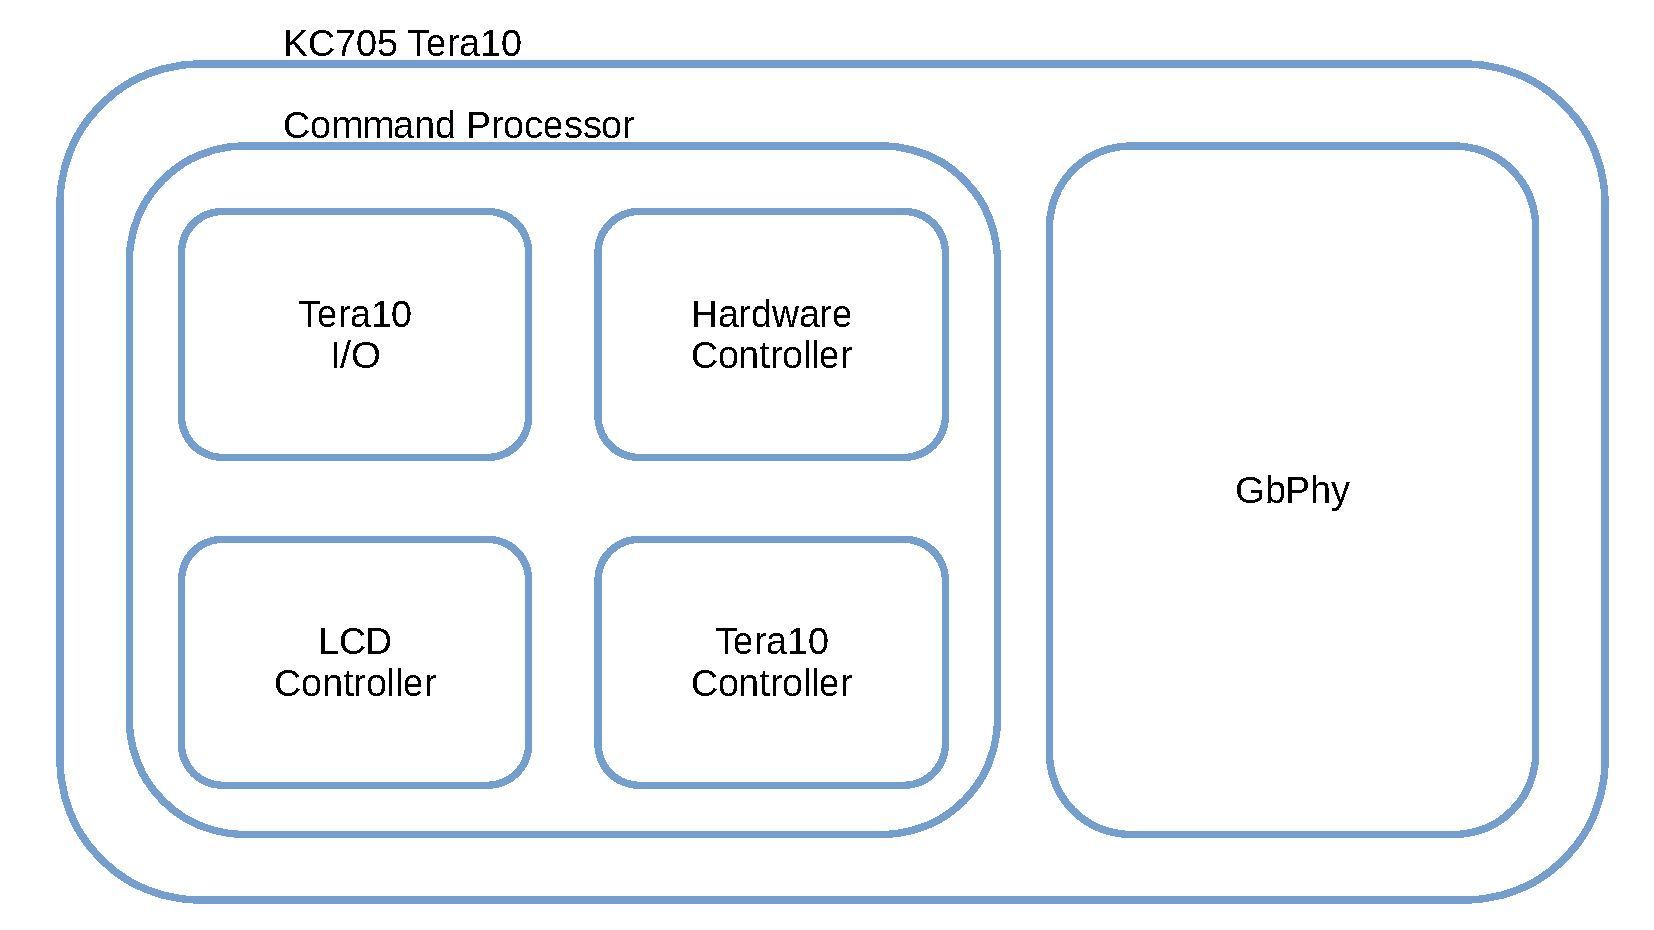
\includegraphics[width=0.7\linewidth]{IMG/ch4/TERA10}
	\caption{KC705 tera10 firmware structure}
	\label{fig:tera10}
\end{figure}
\begin{itemize}
	\item \textbf{KC705 TERA10}: this is the main module, everything lives inside it, thus it contains no logic, only component declarations and port-maps. In this module can be set the firmware version ("B20C" for example) that will the displayed on the LCD.
	%%%%%%%%%%%%%%%%%%%%%%%%%%%%%%%%%%%%%%%%%%%%%%%%%%%%%%%%%%%%%%%%%%%%%%%%%%
	\item \textbf{GbPhy}: the communication between FPGA and computer is done via Ethernet cable using a UDP (User Datagram Protocol). This is done via firmware and also thanks to a dedicated chip connected on the board to the RJ45 connector called "PHY".
	\newline
	PHY is an abbreviation for "physical layer" and is an electronic circuit, usually implemented as a chip (integrated circuit) mandatory to implement links between physical mediums such as copper or optical fiber. It basically converts data between a "clean" clocked digital stream form that is suitable only for very short distance communication (centimetres) and an analog form that is suitable for long range transmission (meters or more).
	The chip on the KC705 board is able to transmit data up to 1Gb/s.
	\newline
	The PHY is thus firmware controlled, in the MoVe\_IT project the reception and sending of messages is managed by another project of the Turin INFN group called GbPhy. This thesis will  not focus on how it works, but only on its main characteristics\cite{gbphy}.     
	\begin{figure}[H]
		\centering
		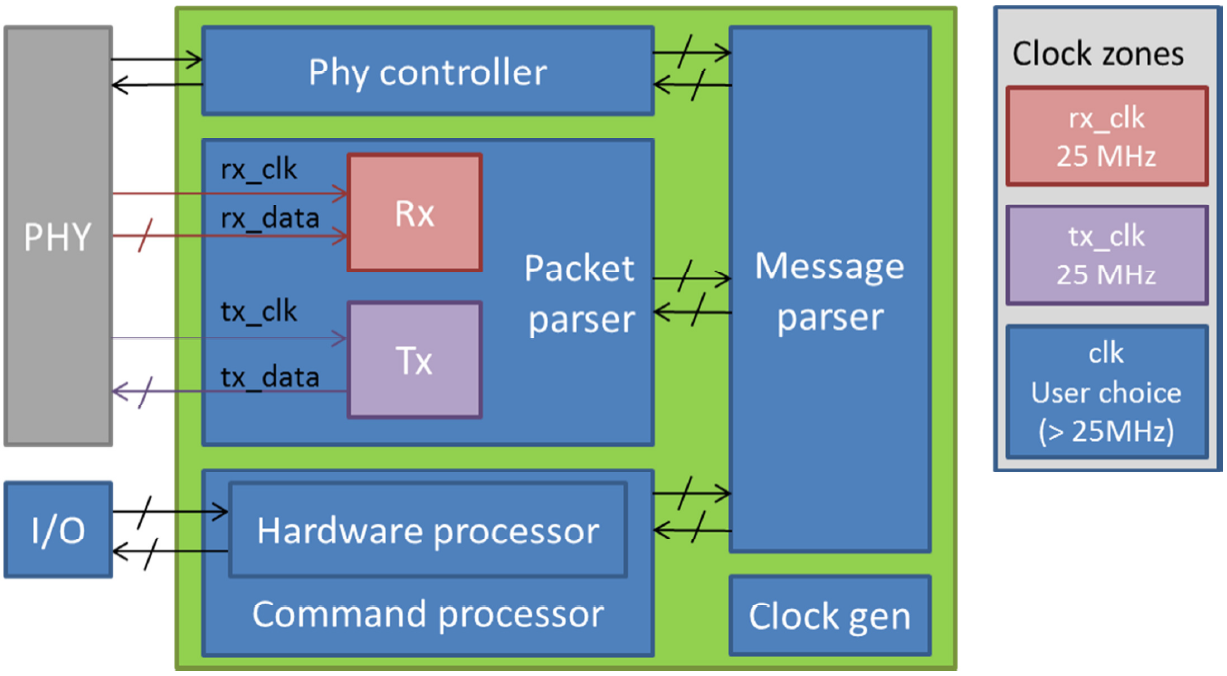
\includegraphics[width=0.7\linewidth]{IMG/ch4/PHY100}
		\caption{GbPhy firmware structure}
		\label{fig:phy100}
	\end{figure}
	\noindent GbPhy provides a UDP-based Ethernet control link based on a fixed length 8 byte protocol.
	For each 8 byte message the user can send 4 bytes of data. The data is thus divides as follow:
	\begin{itemize}
		\item command\_contents(31 downto 28) => sub-system target;
		\newline
		For this application this can be x"1" for hardware commands, x"2" for LCD commands and x"4" for Tera10 commands.
		\item command\_contents(27 downto 20) => sub-system command id;
		\newline
		Each task (or command) has an id, a name with which it can be called, an example of this is the list of commands in the \textit{Tera10 Controller} part in the next pages.
		\item command\_contents(19 downto 0) => sub-system command data;
		\newline
		This 20 bits are the data that may be needed to the firmware; for example, this can be the value of a DAC that needs to be set, or it can be a list of channels that the user wants to enable or it can also be the value of a counter that the user want to read. 
	\end{itemize} 
	%%%%%%%%%%%%%%%%%%%%%%%%%%%%%%%%%%%%%%%%%%%%%%%%%%%%%%%%%%%%%%%%%%%%%%%%%% 
	\item \textbf{Command Processor}: this module is mainly a wrapper for every module that will be presented from now on. It also 
	redirects the commands in accord with the sub-system target.
	%%%%%%%%%%%%%%%%%%%%%%%%%%%%%%%%%%%%%%%%%%%%%%%%%%%%%%%%%%%%%%%%%%%%%%%%%%
	\item \textbf{LCD Controller}: it is the module that drives the 16x2 LCD display of the board.
	\begin{figure}[H]
		\centering
		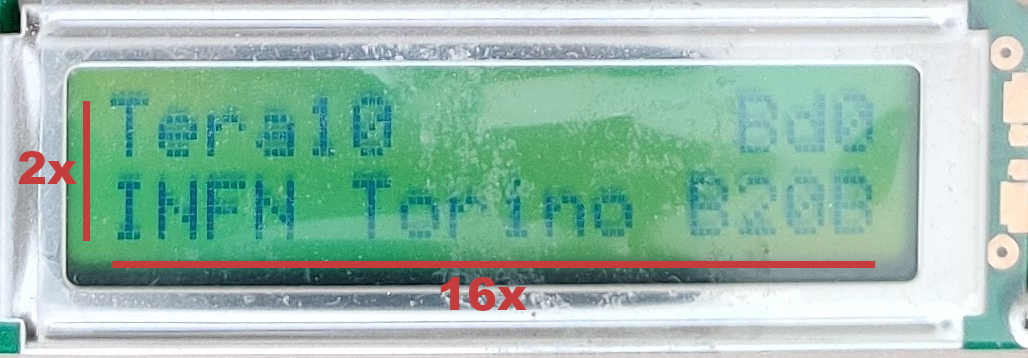
\includegraphics[width=0.5\linewidth]{IMG/ch4/LCD}
		\caption{KC705 tera10 LCD output}
		\label{fig:lcd}
	\end{figure}
	\noindent This module contains multiple processes, FSMs (Finite State Machines) and a RAM module. The first FSM manages the start-up sequence for the LCD, the second does the conversion of the firmware version from hex to ASCII, a third one sends one by one the characters to the display while a fourth one manages the communications with the UDP module. In fact the firmware can not only display a fixed pre-selected banner, but also a user-sent 'message' from the pc.
	The LCD is extremely useful when working with more than one card for discriminating one from another and for keeping track of the firmware version of each board.
	%%%%%%%%%%%%%%%%%%%%%%%%%%%%%%%%%%%%%%%%%%%%%%%%%%%%%%%%%%%%%%%%%%%%%%%%%%    
	\item \textbf{Tera10 I/O}: this module contains the declaration and port-map for 24 \textit{tera10 channel coincidence} modules\cite{limardi}; each module receives as an input the data from two channels of the ABACUS2 chip, this signal is thus de-serialized with a 1GHz frequency (\textit{serdes\_clk}), ten times higher than the main clock (100MHz). The output of the de-serializer is a 10 bit bus (one for each signal) to which it is added, using a shift register, the last bit from the previous bus. This is done in order to not lose any transition (high/low) from one packet and the next one.
	\newline
	The counting of the number of pulses is done with a LUT (Look Up Table) that from a 11bit bus gives back a 3bit logic vector corresponding to the number from 0 to 1. This result is used to update a 32bit counter for each channel; in figure \ref{fig:coincidence} those are N1 for ch0 and N2 for ch1.
	\newline
	In order to count with efficiency even at high rates a previous student implemented in the firmware pile-up correction algorithms. AND and OR logic combinations between the two channels 10bit bus are done, compared with others LUTs and added to four new 32bit counters ($N_{AND}$, $T_{AND}$, $N_{OR}$ and $T_{OR}$). 
	\begin{figure}[H]
		\centering
		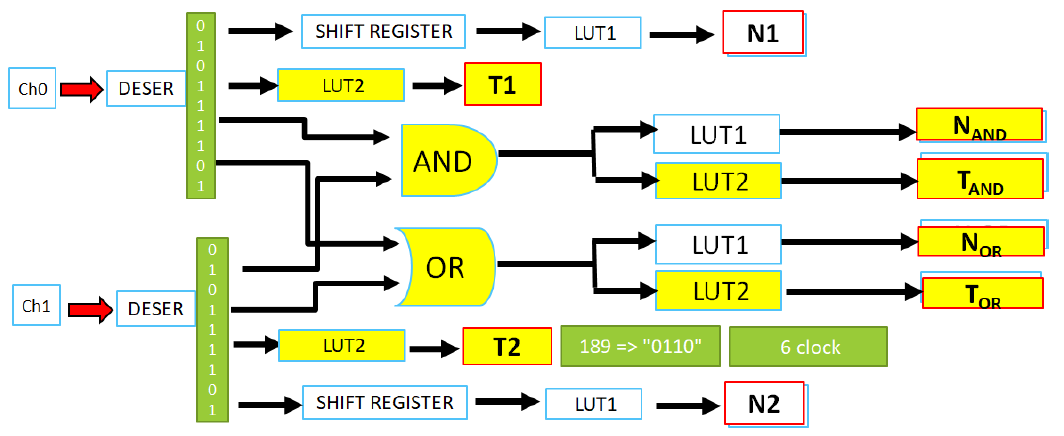
\includegraphics[width=0.7\linewidth]{IMG/ch4/COINCIDENCE}
		\caption{KC705 tera10 channel coincidence architecture diagram}
		\label{fig:coincidence}
	\end{figure}
	\noindent The counters $T_{1}$, $T_{2}$, $T_{AND}$ and $T_{OR}$ contain the number of clock strokes in which one of the two channel or a logic combination of both is \textit{high}.
	%%%%%%%%%%%%%%%%%%%%%%%%%%%%%%%%%%%%%%%%%%%%%%%%%%%%%%%%%%%%%%%%%%%%%%%%%% 
	\item \textbf{Tera10 Controller}: this module is strictly connected to the previous one (\textit{Tera10 I/O}), in fact it receives every counter from the previous block and manages the data in accord to the commands sent by the user. Some of the more used and important commands are:
	\begin{itemize}
		\item x"01" \textit{reset serdes}: send reset signal for the de-serializer.
		\item x"02" \textit{reset counters}: every counter for each \textit{tera10 channel coincidence} module is set to 0.
		\item x"10" \textit{set counter enable}: to enable selected counters. This is done by dividing the channels in blocks of 16. When a 20bit data command is sent bits 18-17-16 are used to identify the block, and the next 16bit are encoded one-hot for each channel; for example, to enable channel 2 the data to be sent is \textit{0-000-0000000000000010} and to enable channel 18 the data is \textit{0-001-0000000000000100}.   
		\item x"11" \textit{read counter}: read selected counter; the firmware response is a 16bit bus, thus 2 commands are needed in order to read the entire counter; the LSB (Least Significative Bit) selects between the fist and last 16bit. For example:
		\newline
		fifo\_data(7 downto 0) = "01110110" means read ch59\_counter(15 downto 0)
		\newline
		fifo\_data(7 downto 0) = "01110111" means read ch59\_counter(31 downto 15)
		\item x"13" \textit{read clocks}: read selected clock counter; the firmware response is a 16bit bus, thus are valid the same considerations as before.
		\item x"14" \textit{read coincidence counter}: read selected coincidence counter, the MSB (Most Significative Bit) selects between \textit{AND} and \textit{OR} counters; the firmware response is a 16bit buss. for example:
		\newline
		fifo\_data(7 downto 0) = "10000010" means read ch0203\_or\_counter(15 downto 0)
		\item x"15" \textit{read coincidence clocks}: read selected clock coincidence counter, the MSB (Most Significative Bit) selects between \textit{AND} and \textit{OR} counters; the firmware response is a 16bit bus.
		%\item x"18" \textit{set selected channel}:
		%\item x"20" \textit{do external trigger}:
		%\item x"12" \textit{read event buffer ram address}:
		%\item x"80" \textit{read event buffer ram}:
	\end{itemize}
	
	%%%%%%%%%%%%%%%%%%%%%%%%%%%%%%%%%%%%%%%%%%%%%%%%%%%%%%%%%%%%%%%%%%%%%%%%%% 
	\item \textbf{Hardware Controller}: this module manages hardware devices such as internal and external DACs, LEDs and GPIO (General Purpose Input Output) switches\&buttons. The main commands are:
	\begin{itemize}
		\item x"01" \textit{read GPIO switches}: this command returns the current state of the GPIO switches and buttons, thus:
		\newline
		reply(8 downto 4) = buttons state
		\newline
		reply(3 downto 0) = switches state
		\item x"02" \textit{set hardware LED}: this command can turn on or off LEDs.
		\item x"11" \textit{set baseline DACs}: this command is used both, for writing (setting) and reading the values of the ABACUS2 internal DACs, this will be explained in detail in section \ref{InternalDac}.
		\item {\color{red} non so se ho detto cose sbagliate}
		\item x"20" \textit{clear external DAC}: to clear the present settings of the eternal DAC. 
		\item x"21" \textit{set external DAC data register}: to set the external DAC with the values written in the RAM.
		\item x"22" \textit{write external DAC register}: to write on RAM the values to be written on the eternal DAC.
	\end{itemize}  
		
\end{itemize}

\section{Firmware update}

\subsection{Hardware controller}\label{InternalDac}
\begin{figure}[H]
	\centering
	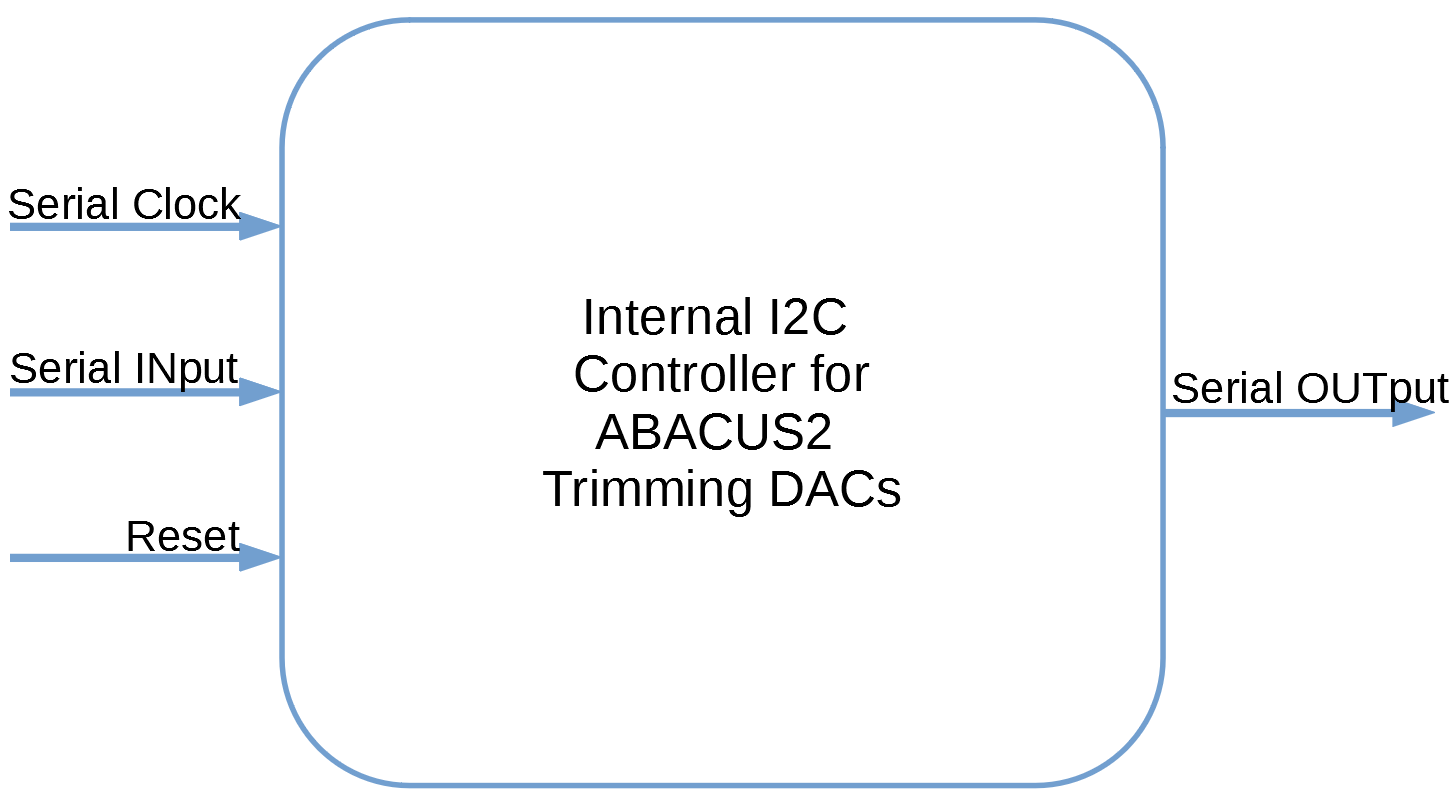
\includegraphics[width=0.5\linewidth]{IMG/ch4/INTERNALDAC}
	\caption{test bench}
	\label{fig:internaldac}
\end{figure}

\begin{figure}[H]
	\centering
	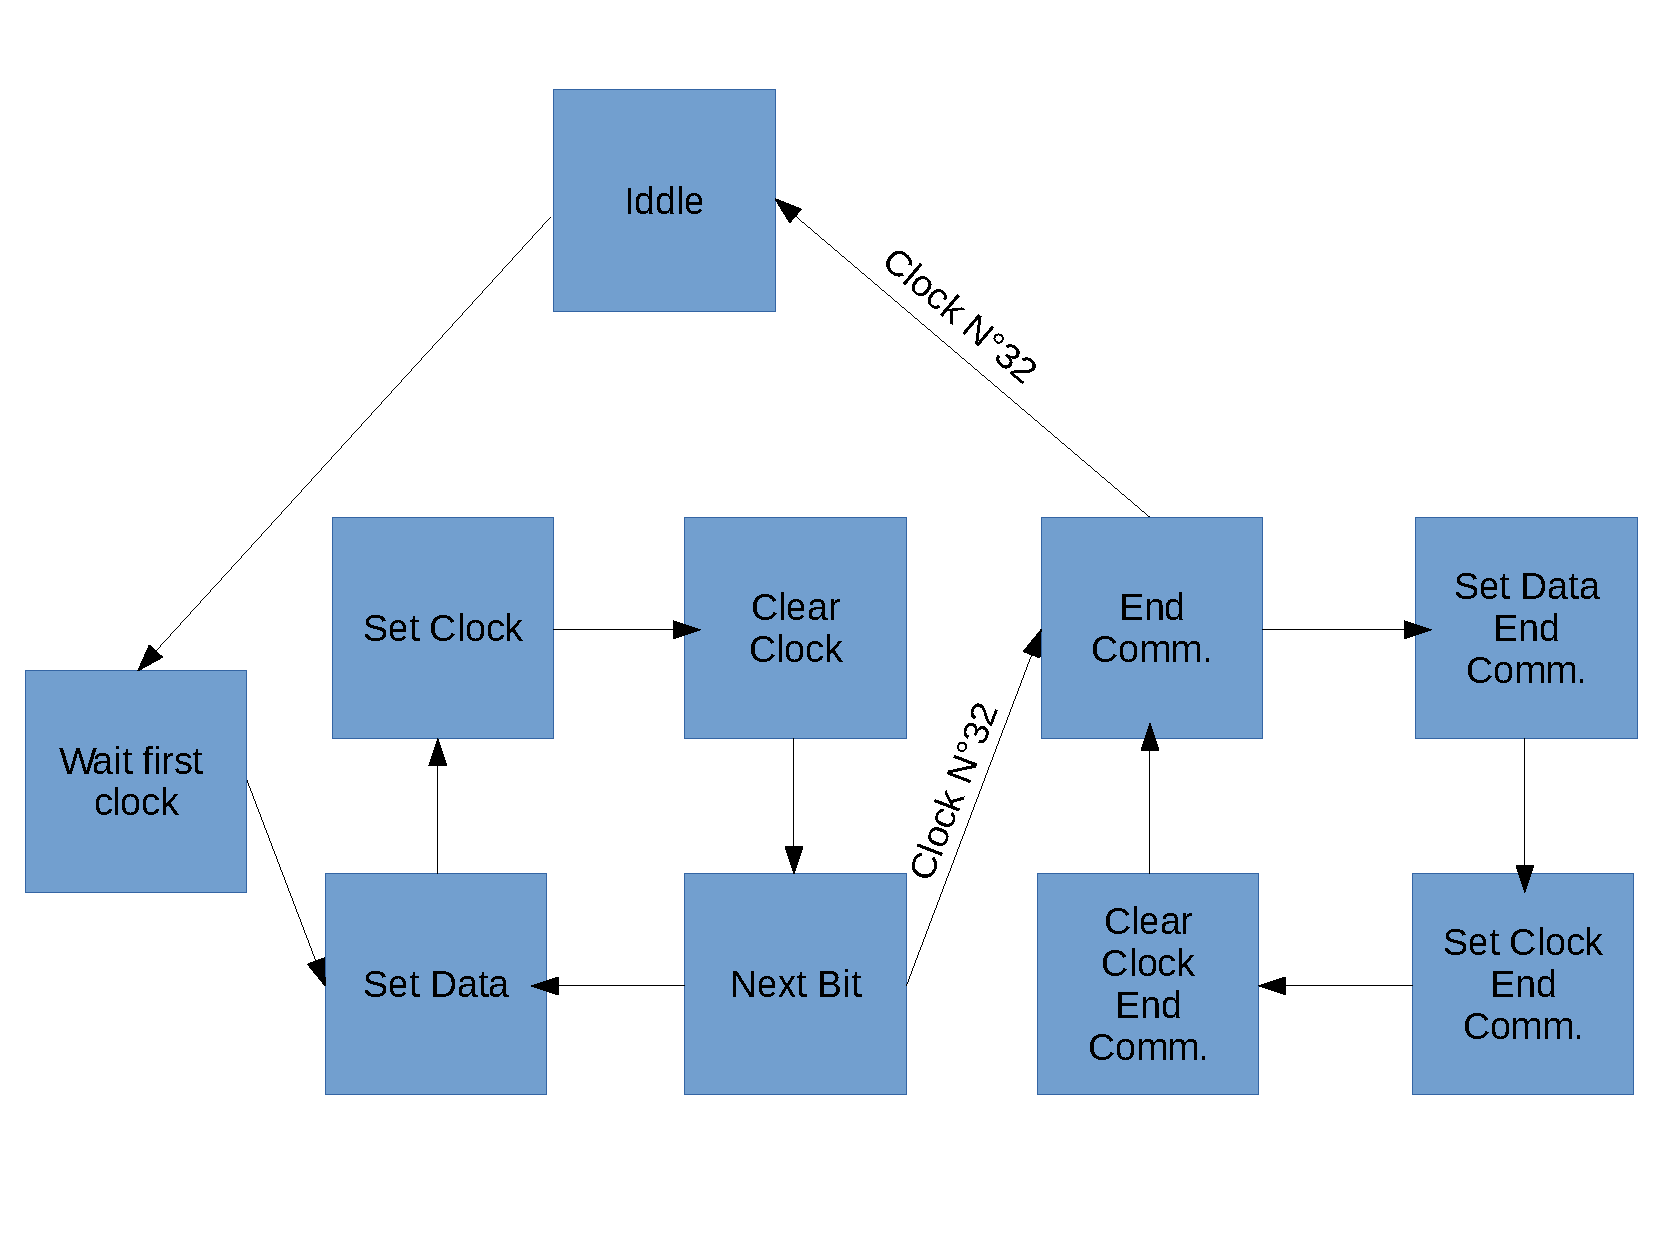
\includegraphics[width=0.7\linewidth]{IMG/ch4/FSM}
	\caption{test bench}
	\label{fig:fsm}
\end{figure}

\subsection{Latching counters}

\subsection{Timestamp generator}

\section{Simulations}

\subsection{Internal DAC simulation}

\subsection{Latching counters simulation}

\subsection{Timestamp generator simulation}

\section{Hardware devices}\label{hardware}

\begin{figure}[H]
	\centering
	\includegraphics[width=0.7\linewidth]{IMG/ch4/DIAGRAM}
	\caption{test bench}
	\label{fig:diagram}
\end{figure}


\section{Test Bench}\label{testbench}
\begin{figure}[H]
	\centering
	\includegraphics[width=0.7\linewidth]{IMG/ch4/TESTBENCH}
	\caption{test bench}
	\label{fig:testbench}
\end{figure}

\section{Test board}\label{testboard}
\begin{figure}[H]
	\centering
	\includegraphics[width=0.7\linewidth]{IMG/ch4/TESTBOARD}
	\caption{test board}
	\label{fig:testboard}
\end{figure}

\section{Esa-Abacus}

	
	\chapter{Experimental setup and tests on board}

\section{Simulations}

\subsection{Internal DAC simulation}

\subsection{Latching counters simulation}

\subsection{Timestamp generator simulation}

\section{Hardware devices}\label{hardware}

\begin{figure}[H]
	\centering
	\includegraphics[width=0.7\linewidth]{IMG/ch5/DIAGRAM}
	\caption{test bench}
	\label{fig:diagram}
\end{figure}


\section{Test Bench}\label{testbench}
\begin{figure}[H]
	\centering
	\includegraphics[width=0.7\linewidth]{IMG/ch5/TESTBENCH}
	\caption{test bench}
	\label{fig:testbench}
\end{figure}

\section{Test board}\label{testboard}
\begin{figure}[H]
	\centering
	\includegraphics[width=0.7\linewidth]{IMG/ch5/TESTBOARD}
	\caption{test board}
	\label{fig:testboard}
\end{figure}

\section{Esa-Abacus}
	
	


\newpage
\section*{Conclusions and future developments}
\pagestyle{plain}
\noindent This thesis work was carried out inside the MoVe\_IT project.
Along side my work on the FPGA firmware other students were involved on the chip characterisation, test\&data-analysis of the ESA-ABACUS board and time of flight measurements.
I personally designed, implemented and tested with success three additions to the FPGA firmware that will be used for hadron therapy tests.
In addition, I developed a debug tool for the verification of the working conditions of the FPGA channels.
My job started with an already working project created by \textit{Richard Wheadon} and updated by \textit{Alessio Limardi}.
For the lab tests I was helped by INFN researcher \textit{Simona Giordanengo} and thesis student \textit{Emanuele Data}.
In this elaborate it was shown:
\begin{itemize}
	\item A new configuration logic for the internal (trimming) DACs of the ABACUS\_v2 chip, in section \ref{InternalDac}.
	\item The creation of a latch system that generates a "picture" of the state of every counter and the new commands to reads this saved data, in section \ref{Latch}
	\item The implementation of a 64 bit timestamp used to obtain a more precise measurement of the particle rate, section \ref{Timestamp}
\end{itemize}
\noindent All these additions were tested within chapter 5 with positive results.
The main goal for the future is to write an optimized and fully capable data acquisition panel with LabVIEW able of using at his full extend the new features of the FPGA.  
From section \ref{UtilizationReport} it emerges that the KC705 board is underused, thus many more additions could be implemented; the most important ones could be:
\begin{itemize}
	\item The creation of a software configurable mask that allows the hardware calculation of the sum of the counts of only the selected channels.  
	\item The implementation of the particle rate calculation directly on board.
\end{itemize}


\chapter*{Greetings}
\vspace*{3cm}
\noindent I would like to dedicate this thesis to my parents, \textit{Cristina Staviri} and \textit{Nicolae Zugravel} who have always supported me during my university career.
They kept me in Turin for five years and never put pressure on me.
A thought of mine goes to my partner \textit{Giorgia Rista} on whom I have always been able to count.
I would like to sincerely thank my supervisor \textit{Luca Pacher} who has always helped me and inspired to do better.
My thanks also go to my co-supervisor Professor \textit{Vincenzo Monaco} who has always been available for all my questions and to researcher \textit{Simona Giordanengo} who helped me a lot during the validation process.
Finally, my thoughts go to all my friends, both those I met at the university and those I met many years before.
Working for this project has been a pleasure and an experience that has taught me a lot.
I can't wait to continue my journey and improve myself more and more.
To conclude, I would like to thank one last time whoever has read this thesis work, I hope you have enjoyed reading it and that you have found it interesting as much as I did.\\
\noindent Sincerely.
\vspace*{1cm}
\begin{flushright}
	\textit{Stefan Cristi Zugravel}
\end{flushright}
	
	\begin{thebibliography}{00}	
	\bibitem[1]{tumor}www.medicalnewstoday.com/articles/249141
	\bibitem[2]{radiationtherapy}enlight.web.cern.ch/what-is-hadron-therapy
	\bibitem[3]{landau}L. Landau, On the Energy Loss of Fast Particles by Ionization, Journal of
	Physics 8, (1944), 201 -205
	\bibitem[4]{cells}H. Tsujii et al., Carbon-Ion Radiotherapy – Principles, Practices and Treatment
	Planning, Springer, (2012)
	\bibitem[5]{let}D. Schardt, T. Elsasser, Heavy-ion tumor therapy: Physical and radiobiological
	benefits, Reviews of Modern Physics, 82, (2010)
	\bibitem[6]{cnao}Giordanengo et al., Design and characterization of the beam monitor detectors
	of the Italian National Center of Oncological Hadron-therapy (CNAO).
	\bibitem[7]{pencil}S. Giordanengo et al , The CNAO Dose Delivery System for ion pencil beam
	scanning radiotherapy, Medical Physics (2015)
	\bibitem[8]{detector}Hartmann, F., Silicon tracking detectors in high energy physics, Nucl.Instr.Meth.A
	666 (2012) 25-46.
	%----------------------------------------------------------------------
	\bibitem[9]{moveit}MoVe\_IT, Modeling and Verification for Ion beam Treatment planning, INFN CSN5 “Call 2017” Project proposal
	\bibitem[10]{lgad}G. Pellegrini et al, Technology developments and first measurements of Low Gain Avalanche Detectors (LGAD) for high energy physics applications, Nucl.Instrum.Meth. A765 (2014) 12-16.
	\bibitem[11]{abacus}A single ion discriminator ASIC prototype for particle therapy applications
	\bibitem[12]{hammad}CHARACTERIZATION AND TEST OF LGAD STRIP SILICON DETECTORS TO COUNT THE NUMBER OF PROTONS OF THERAPEUTIC BEAMS, Omar Hammad Ali
	%----------------------------------------------------------------------
	\bibitem[13]{fpga1}Introduction to FPGA design, J. Serrano, CERN-Geneva-Switzerland
	\bibitem[14]{fpga2}Three Ages of FPGAs: A Retrospective on the First Thirty Years of FPGA Technology, By Stephen M. (Steve) Trimberger, Fellow IEEE
	\bibitem[15]{fpga3}Introduction to Field Programmable Gate Arrays Hannes Sakulin CERN / EP-CMD
	\bibitem[16]{fpga4}Field Programmable Gate Arrays and Applications, Version 2 EE IIT, Kharagpur
	\bibitem[17]{hdl}en.wikipedia.org/wiki/Hardware\_description\_language
	\bibitem[18]{vhdl}Free Range VHDL, Bryan Mealy, Fabrizio Tappero
	\bibitem[19]{constraints1}Vivado Design Suite User Guide
	\bibitem[20]{constraints2}Constraints Guide ISE 6.2.03i
	\bibitem[21]{vivado}en.wikipedia.org/wiki/Xilinx\_Vivado
	\bibitem[22]{labview}www.ni.com/pdf/manuals/320999e.pdf
	\bibitem[23]{kintex7}KC705 Evaluation Board for the Kintex-7 FPGA	
	\bibitem[24]{tcl}www.tcl.tk
	\bibitem[25]{lvds}en.wikipedia.org/wiki/Low-voltage\_differential\_signaling
	%----------------------------------------------------------------------
	\bibitem[26]{gbphy}personalpages.to.infn.it/~wheadon/fpga/phy100/default.html
	\bibitem[27]{dac}MoveIt v2 design document, Giovanni Mazza, January 15 2021
	\bibitem[28]{timing}www.eejournal.com/article/20130528-timing/
	\bibitem[29]{limardi}Sviluppo su FPGA di tecniche di correzione di effetti d'inefficienza nel conteggio di singoli protoni in fasci terapeutici, Alessio Limardi, 2019-2020.
	%----------------------------------------------------------------------
	\bibitem[30]{LTC2604}www.analog.com/media/en/technical-documentation/data-sheets/2604fd.pdf
	\bibitem[31]{data}Emanuele Data's masters degree thesis 
	
	
\end{thebibliography}

	
\end{document}